\documentclass[11pt]{amsart}
\usepackage[T1]{fontenc}
\usepackage[utf8]{inputenc}
\usepackage{lmodern}
\usepackage[letterpaper,margin=1in]{geometry}
\usepackage{amsmath,amssymb,mathtools}
\usepackage{booktabs,longtable,array}
\usepackage{enumitem}
\usepackage{microtype}
\usepackage{xcolor}
\usepackage{graphicx}
\graphicspath{{figures/}{source_archive/}}
\usepackage{listings}
\lstset{basicstyle=\ttfamily\scriptsize,breaklines=true,columns=fullflexible,frame=single}
\usepackage[colorlinks=true,linkcolor=blue!45!black,citecolor=blue!45!black,urlcolor=blue!45!black]{hyperref}

\newtheorem{theorem}{Theorem}[section]
\newtheorem{proposition}[theorem]{Proposition}
\newtheorem{lemma}[theorem]{Lemma}
\newtheorem{corollary}[theorem]{Corollary}
\newtheorem{hypothesis}[theorem]{Hypothesis}
\theoremstyle{definition}
\newtheorem{definition}[theorem]{Definition}
\theoremstyle{remark}
\newtheorem{remark}[theorem]{Remark}

\newcommand{\dd}{\,\mathrm d}
\newcommand{\ee}{\mathrm e}
\newcommand{\RH}{\mathrm{RH}}
\newcommand{\Off}{\operatorname{Off}}
\newcommand{\supp}{\operatorname{supp}}
\newcommand{\Log}{\operatorname{Log}}
\newenvironment{numericalcheck}
{\begin{quote}\small\noindent\textbf{Numerical compatibility.}\ }{\end{quote}}

\title[Exponential centroids and pair correlation]{Exponential Centroids and Montgomery's Pair-Correlation Conjecture\\
Exact inversion, the archimedean carrier spectrum, and the residual plateau problem}
\author{Víctor Casaña-Giner}
\thanks{Bio Logic Crop Science S.L., E-46120 Alboraya (Valencia), Spain. E-mail: \texttt{vcasana@biologiccropscience.com}. ORCID: 0000-0002-8252-2608.}
\date{August 2026}

\begin{document}

\begin{abstract}
Let $0<\gamma_1\leq\gamma_2\leq\cdots$ be the positive ordinates of the
nontrivial zeros of the Riemann zeta function, counted with multiplicity, and
let
\[
S_N(u)=\sum_{k\leq N}\ee^{iu\gamma_k},
\qquad
C_N(u)=\frac1N\sum_{n\leq N}S_n(u).
\]
The starting statistic is the complex exponential-walk centroid $C_N(1)$.  We
first record the conditional analytic limit previously obtained from the
one-sided explicit formula and prove two fixed-frequency pair-cancellation
identities forced by the walk and its centroid.  The frequency family loses no
spectral information: if $A_N(u)=NC_N(u)$, then
$\Delta A_N(u)=S_N(u)$ and $\Delta^2A_N(u)=\ee^{iu\gamma_N}$.  Consequently an
exponentially smoothed square of $\Delta A_N$ is exactly Montgomery's weighted
form factor.  Under RH this gives Montgomery's full proved ramp through
$|\alpha|=1$ and, by Fourier inversion, the sine-kernel law for band-limited
tests.

We then unfold by the smooth Riemann--von Mangoldt clock
$M(t)=\frac{t}{2\pi}\log\frac{t}{2\pi\ee}+\frac78$ and set
$\eta_k=M(\gamma_k)-(k-\frac12)$.  Every unfolded pair separation satisfies the
exact identity
\[
M(\gamma_{k+h})-M(\gamma_k)=h+\eta_{k+h}-\eta_k.
\]
Thus the full sine law is precisely an increment law for the residual sequence
$\eta_k$.  The synthetic Lambert carrier $M(\tau_k)=k-\frac12$ supplies an exact
counterexample to the implication ``centroid convergence implies GUE pairs'':
its centroid converges at rate $O(\log^2N/N)$, while its unfolded pair measure
is a Dirac comb.  Poisson summation gives its closed archimedean saddle
spectrum, with saddles $\tau=2\pi\ee^{t/n}$ and leading amplitude
$t\ee^{t/(2n)}n^{-3/2}$.

Finally, the remaining Montgomery plateau is isolated as residual
off-diagonal decorrelation.  In the truncated Selberg prime model we prove the
needed twisted quadratic cancellation for $0<\alpha<2$; the only remaining
transfer is the oscillatory contribution of the Selberg remainder.  Independent
computations with $22{,}491$ ordinates reproduce the sine density, the connected
form factor, and the empirical $\log N/N$ centroid rate, whose 90-fold
extrapolation agrees in scale and value with the independent
$N=2{,}001{,}052$ computation.
\end{abstract}

\maketitle

\noindent\textbf{Keywords.} Riemann zeta function; exponential centroid;
Montgomery pair correlation; GUE; sine kernel; Riemann--von Mangoldt clock;
Lambert $W$; stationary phase; Selberg polynomial.

\medskip
\noindent\textbf{MSC 2020.} 11M06; 11M26; 11M36; 60B20.

\tableofcontents

\section{Analytic domain, regularity, and endpoint conventions}
\label{sec:conventions}

The meromorphic continuation of $\zeta(s)$ is used on $\mathbb C$: it has one
simple pole at $s=1$, trivial zeros at the negative even integers, and its
nontrivial zeros lie in $0<\Re s<1$.  Write
$\rho_k=\beta_k+i\gamma_k$, $\gamma_k>0$, for all upper-half-plane
nontrivial zeros, ordered by nondecreasing ordinate and repeated according to
algebraic multiplicity.  Equal ordinates therefore occupy distinct ordinal
slots.  RH is the assertion $\beta_k=1/2$ for every $k$.

For real $t>0$ set
\begin{equation}\label{eq:theta_exact}
\vartheta(t)=\Im\Log\Gamma\!\left(\frac14+\frac{it}{2}\right)
-\frac t2\log\pi,
\qquad H(t)=1+\frac{\vartheta(t)}{\pi}.
\end{equation}
The branch of $\Log\Gamma$ is the continuous branch obtained from $t=0$.
The line $1/4+it/2$ meets neither a pole nor a zero of $\Gamma$; hence
$\vartheta$ and $H$ are real analytic on $(0,\infty)$.  In particular,
\begin{equation}\label{eq:H_derivatives}
H'(t)=\frac1{2\pi}\Re\psi\!\left(\frac14+\frac{it}{2}\right)
-\frac{\log\pi}{2\pi},
\qquad H'(t)=O(\log(2+t)),\quad H''(t)=O((1+t)^{-1}).
\end{equation}

The counting function $\mathcal N(t)=\#\{k:0<\gamma_k\le t\}$ is
right-continuous.  Away from zero ordinates define $S(t)=\mathcal N(t)-H(t)$.
If a distinct ordinate $\gamma$ has multiplicity $\nu(\gamma)$, put
\begin{equation}\label{eq:midpoint_precise}
\mathcal N_*(\gamma)=\frac{\mathcal N(\gamma^-)+\mathcal N(\gamma^+)}2,
\qquad S_*(\gamma)=\mathcal N_*(\gamma)-H(\gamma).
\end{equation}
Lebesgue integrals are unchanged by the chosen values at jumps.  Stieltjes
integrals use the midpoint value in \eqref{eq:midpoint_precise}; thus, for a
jump of arbitrary size, $S_*\,\dd S=\tfrac12\dd(S^2)$ exactly.  A height
endpoint is first completed to the entire multiplicity block; an ordinal
endpoint inside that block is then obtained by removing the unused repeated
slots.  The correction is $O(\nu(\gamma)^2)$ and
$\nu(\gamma)=O(\log(2+\gamma))$.

The smooth main clock
\begin{equation}\label{eq:M_domain}
M(t)=\frac{t}{2\pi}\log\frac{t}{2\pi\ee}+\frac78
\end{equation}
is $C^\infty$ for $t>0$ and strictly increasing for $t>2\pi$, since
$M'(t)=(2\pi)^{-1}\log(t/2\pi)>0$.  Every equation
$M(\tau_k)=k-1/2$, $k\ge1$, has one and only one solution in $(2\pi,\infty)$.
The Lambert formula used below employs the real principal branch $W_0$.  Its
arguments $(k-11/8)/\ee$ lie in $(-1/\ee,\infty)$ and never equal zero, so
$W_0$ is real and the quotient has no branch singularity or zero denominator.

All finite sums and finite differences are algebraic and require no limiting
interchange.  Fubini or Fourier inversion is used only after absolute
integrability has been stated.  A numerical check establishes finite-data
compatibility, never an asymptotic theorem.  Exact identities are reported by
their floating-point closure error; conjectural or conditional steps retain
their hypotheses explicitly.

\section{The exponential walk and its centroid}

For $u\in\mathbb R$ define
\begin{equation}\label{eq:walk_centroid}
S_N(u):=\sum_{k\leq N}\ee^{iu\gamma_k},
\qquad
C_N(u):=\frac1N\sum_{n\leq N}S_n(u)
=\sum_{k\leq N}\left(1-\frac{k-1}{N}\right)\ee^{iu\gamma_k}.
\end{equation}
The statistic that motivated the work is $C_N(1)$.  Its real and imaginary
coordinates retain an orientation which disappears from a modulus or from a
pair-difference statistic.

The counting objects and their midpoint convention are those of
Section~\ref{sec:conventions}.  For an index in the block at $\gamma$, define
$r_k=k-\tfrac12-H(\gamma_k)$.  If that block begins after $a$ earlier slots,
then direct summation gives
\begin{equation}\label{eq:block_defect}
\sum_{j=1}^{\nu(\gamma)}r_{a+j}=\nu(\gamma)S_*(\gamma).
\end{equation}

\begin{theorem}[Level-one reduction]\label{thm:level_one}
Let
\[
Q_N^{(H)}:=\frac1N\sum_{k\leq N}
\left(N+\frac12-H(\gamma_k)\right)\ee^{i\gamma_k}.
\]
Then
\begin{equation}\label{eq:level_one}
C_N(1)-Q_N^{(H)}\longrightarrow0
\end{equation}
unconditionally.
\end{theorem}

\begin{proof}
The exact triangular identity gives
\begin{equation}\label{eq:CQ_exact}
C_N(1)-Q_N^{(H)}=-\frac1N\sum_{k\le N}r_k\ee^{i\gamma_k}.
\end{equation}
We first end at a complete ordinate block $T$ which is not itself a zero and
put
\[
A(T)=\sum_{\substack{\gamma\le T\\\gamma\ {
m distinct}}}
\nu(\gamma)S_*(\gamma)\ee^{i\gamma}
=\int_{0^-}^{T}\ee^{it}S_*(t)\,\dd\mathcal N(t),
\]
where the last equality follows from \eqref{eq:block_defect}.  Since $H$ is
$C^1$ and $S$ has locally bounded variation,
$\dd\mathcal N=H'(t)\dd t+\dd S(t)$.  Midpoint Stieltjes integration by parts
therefore gives, with bounded lower-end terms absorbed in $O(1)$,
\begin{equation}\label{eq:level_one_core}
A(T)=\frac12\ee^{iT}S(T)^2
-\frac{i}{2}\int_0^T\ee^{it}S(t)^2\,\dd t
+\int_0^T\ee^{it}H'(t)S(t)\,\dd t+O(1).
\end{equation}

Here the Selberg input is used in exactly one place: for $T\ge3$,
\begin{equation}\label{eq:Selberg_exact_use}
\int_0^T|S(t)|^2\,\dd t\ll T\log\log T.
\end{equation}
The function $S$ is measurable and locally bounded away from its countable
set of jumps, so it lies in $L^2(0,T)$ and the integral exists.  Because
$|\ee^{it}|=1$, \eqref{eq:Selberg_exact_use} implies
\[
\left|\int_0^T\ee^{it}S(t)^2\dd t\right|
\le\int_0^T|S(t)|^2\dd t\ll T\log\log T=o(T\log T).
\]
Also $S(T)=O(\log T)$ gives the endpoint $O(\log^2T)$.

The remaining linear term is not a consequence of Selberg's estimate.  Put
\[
B(T)=\sum_{0<\gamma_k\le T}\ee^{i\gamma_k},
\qquad F(T)=\int_0^T\ee^{it}S(t)\dd t.
\]
Stieltjes integration by parts, first on intervals avoiding zero ordinates and
then by passage to the endpoint, gives
\begin{equation}\label{eq:F_identity_detailed}
iF(T)=\ee^{iT}S(T)-B(T)+\int_0^T\ee^{it}H'(t)\dd t+O(1).
\end{equation}
Ford--Zaharescu's second-order equidistribution theorem
\cite{FordZaharescu2005} is applied with the
$C^2(\mathbb T)$ test $f(u)=\ee^{2\pi iu}$ and
$\alpha=(2\pi)^{-1}$.  Its mean term vanishes.  Its secondary term is also
zero because resonance would require $1=(a/q)\log p$, equivalently
$\ee=p^{a/q}$, impossible for integers $p,a,q$.  Thus
$B(T)=o(T)$, zeros being counted with multiplicity.  Moreover
\eqref{eq:H_derivatives} and ordinary integration by parts give
$\int_0^T\ee^{it}H'(t)\dd t=O(\log T)$.  Equation
\eqref{eq:F_identity_detailed} yields $F(T)=o(T)$.

Since $F$ is absolutely continuous and $H'$ is $C^1$, a second ordinary
integration by parts is legitimate:
\[
\int_0^T\ee^{it}H'(t)S(t)\dd t
=H'(T)F(T)-\int_0^T H''(t)F(t)\dd t+O(1).
\]
The endpoint is $o(T\log T)$.  Given $\varepsilon>0$, choose $T_0$ so that
$|F(t)|\le\varepsilon t$ for $t\ge T_0$; then
$\int_{T_0}^T|H''(t)F(t)|\dd t\ll\varepsilon T$, while the initial integral is
constant.  Hence this linear term is $o(T\log T)$.  Substitution in
\eqref{eq:level_one_core} proves $A(T)=o(T\log T)$.

If the ordinal cutoff $N$ stops inside its last multiplicity block, completion
changes the numerator in \eqref{eq:CQ_exact} by $O(\log^2(2+\gamma_N))$.
The Riemann--von Mangoldt estimate gives
$N\asymp\gamma_N\log(2+\gamma_N)$, so division by $N$ proves
\eqref{eq:level_one}.
\end{proof}

\begin{numericalcheck}
For the $22{,}491$-ordinate binary,
$C_N=0.777204389314+0.768179110409i$ and
$Q_N^{(H)}=0.777328038812+0.768246161499i$, giving
$|C_N-Q_N^{(H)}|=1.40659\times10^{-4}$.  The first panel of
Figure~\ref{fig:core_checks} shows the finite-height decrease; the midpoint
clock defect has standard deviation $0.297362294$.
\end{numericalcheck}

The one-sided explicit formula supplies the conditional value of the complex
centroid.  For $x_0\in(0,\gamma_1)$ put
\begin{equation}\label{eq:smooth_centroid_term}
\mathcal B(x_0)=\ee^{ix_0}\bigl(H(x_0)+iH'(x_0)\bigr)
+i\int_{x_0}^{\infty}\ee^{it}H''(t)\,\dd t,
\end{equation}
and, for $\sigma>1$,
\begin{align}
\mathcal P_{\sigma}(x_0)
=\frac{i\ee^{ix_0}}{2\pi}\Bigg\{&
\int_0^\infty\ee^{-v}\Log\zeta(\sigma+v-ix_0)\,\dd v\notag\\
&+\int_0^\infty\ee^{v}
\left[\Log\zeta(\sigma+v+ix_0)-2^{-(\sigma+v+ix_0)}\right]\dd v
-\frac{2^{-\sigma-ix_0}}{1-\log2}\Bigg\}.
\label{eq:prime_centroid_term}
\end{align}

\begin{hypothesis}[Boundary interchange]\label{hyp:boundary}
The finite ordinal triangular transform of the argument term has the same
boundary value as
$\lim_{\sigma\downarrow1/2}\mathcal P_\sigma(x_0)$, with the branch of
$\Log\zeta$ continued from $\Re s>1$.
\end{hypothesis}

\begin{theorem}[Complex centroid limit]\label{thm:complex_centroid}
Assume RH and Hypothesis~\ref{hyp:boundary}.  Then
\begin{equation}\label{eq:complex_limit}
C_N(1)\longrightarrow L
=\mathcal B(x_0)+\lim_{\sigma\downarrow1/2}\mathcal P_\sigma(x_0),
\end{equation}
independently of admissible $x_0$.  At $x_0=1$,
\begin{equation}\label{eq:numerical_limit}
L=0.77689426079325358\ldots
+0.767855668864547\ldots i,
\end{equation}
and
\begin{equation}\label{eq:real_limit_closed}
\Re L=\frac1{2\sqrt\ee}\left(\ee-\frac1{\ee^2-1}\right).
\end{equation}
\end{theorem}

\begin{proof}
Theorem~\ref{thm:level_one} reduces the ordinal centroid to a smooth transform
and a linear transform of $S(t)$.  For $\sigma>1$, the Euler product
\[
\frac1\pi\Im\Log\zeta(\sigma+it)
=-\frac1\pi\sum_{n\ge2}\frac{\Lambda(n)}{n^\sigma\log n}
\sin(t\log n)
\]
converges absolutely and locally uniformly in $t$.  Indeed
$\sum_{n\ge2}\Lambda(n)/(n^\sigma\log n)<\infty$, so multiplication by the
bounded triangular kernel and Tonelli's theorem justify termwise integration.
The half-plane $\sigma>1$ contains no zero of $\zeta$ and excludes its pole at
$1$; hence the Euler-product branch of $\Log\zeta$ is holomorphic there.

The two Laplace integrals in \eqref{eq:prime_centroid_term} converge
absolutely.  In the first, $\Log\zeta(\sigma+v-ix_0)=O(2^{-v})$ and the factor
$\ee^{-v}$ strengthens the decay.  In the second, subtraction of the $n=2$
Euler term leaves $O(3^{-v})$; multiplication by $\ee^v$ is integrable because
$\log3>1$.  The denominator $1-\log2$ is nonzero.  The restriction
$0<x_0<\gamma_1$ ensures that the horizontal rays used to continue the branch
meet no nontrivial zero; their nonzero imaginary part also avoids the pole at
$s=1$, and they meet no negative even integer.  The gamma-factor derivatives
in \eqref{eq:smooth_centroid_term} are continuous on $[x_0,\infty)$, while
$H''(t)=O(t^{-1})$ with an oscillatory exponential; integration by parts makes
the improper integral convergent.

The two frequency branches then sum to \eqref{eq:prime_centroid_term} and the
gamma-factor part is \eqref{eq:smooth_centroid_term}.  Nothing in the preceding
absolute-convergence argument reaches $\sigma=1/2$.  Precisely that boundary
passage is Hypothesis~\ref{hyp:boundary}.  Under RH every complete-zero weight
$\ee^{\rho-1/2}$ equals $\ee^{i\gamma}$; off RH it would retain the horizontal
factor $\ee^{\beta-1/2}$.  The symmetric explicit formula at $x=\ee$ gives the
real coordinate; its prime-power distribution has no atom there because
$\ee$ is not an integral prime power.  Direct quadrature gives
\eqref{eq:numerical_limit}.  Independence of $x_0$ follows because two
admissible cutoffs evaluate the same finite triangular transform before the
hypothesized boundary limit.
\end{proof}

\begin{numericalcheck}
At $N=22{,}491$, both coordinates are close to the conditional value:
$|C_N-L|=4.48101\times10^{-4}$, with real and imaginary discrepancies
$3.10129\times10^{-4}$ and $3.23442\times10^{-4}$.  Over 60 logarithmic
cutoffs, $|C_N-L|N/\log N=1.144738\pm0.258893$; see
Figures~\ref{fig:core_checks} and \ref{fig:centroid_rate}.  This is compatible
with the boundary value but does not establish Hypothesis~\ref{hyp:boundary}.
\end{numericalcheck}

\section{Pair cancellation already forced at frequency one}

Put $w_{k,N}=1-(k-1)/N$.  Squaring the complex centroid gives an exact pair
identity.

\begin{proposition}[Triangular pair cancellation from centroid convergence]
\label{prop:centroid_pair_cancel}
If $C_N(1)\to L$, then
\begin{equation}\label{eq:centroid_pair_cancel}
2\sum_{1\leq j<k\leq N}w_{j,N}w_{k,N}
\cos(\gamma_j-\gamma_k)
=-\frac N3+\left(|L|^2-\frac12\right)+o(1).
\end{equation}
\end{proposition}

\begin{proof}
Expansion of $|C_N(1)|^2$ gives a diagonal term
\[
\sum_{k\leq N}w_{k,N}^2
=\frac N3+\frac12+\frac1{6N}.
\]
Subtract this diagonal from $|C_N(1)|^2\to|L|^2$.
\end{proof}

\begin{numericalcheck}
At $N=512$, direct $O(N^2)$ summation of the weighted cosine pairs and the
closed expression $|C_N|^2-\sum w_{k,N}^2$ differ by
$9.66\times10^{-13}$.  At $N=22{,}491$ the remainder after subtracting the
displayed asymptotic main term is $9.71377\times10^{-4}$.
\end{numericalcheck}

There is also an RH-conditional pair theorem which does not assume convergence
of the centroid.  Landau's fixed-real formula, with all zeros in a complete
height block and counted with multiplicity, is
\[
\sum_{0<\gamma\le T}X^\rho
=-\frac{T}{2\pi}\Lambda_{\mathbb R}(X)+O_X(\log T),
\]
where $\Lambda_{\mathbb R}(X)=\log p$ if $X=p^m$ is an integral prime power
and is zero otherwise.  The domain is fixed $X>1$; no uniform limit in $X$ is
used \cite{Landau1912,Gonek}.  At $X=\ee$ the main term is absent.  Under RH,
$\ee^{\rho-1/2}=\ee^{i\gamma}$, and completion/removal of a terminal
multiplicity block costs $O(\log T)$.  Height-to-index transport therefore
yields
\begin{equation}\label{eq:fixed_e_walk_bound}
S_N(1)=O(\log N).
\end{equation}

\begin{theorem}[Trajectory-energy pair cancellation under RH]
\label{thm:trajectory_pair_cancel}
Assume RH.  Then
\begin{equation}\label{eq:trajectory_energy}
\mathcal E_N:=\frac1N\sum_{n\leq N}|S_n(1)|^2=O(\log^2N),
\end{equation}
and consequently
\begin{equation}\label{eq:trajectory_pair_cancel}
2\sum_{1\leq j<k\leq N}
\left(1-\frac{k-1}{N}\right)\cos(\gamma_j-\gamma_k)
=-\frac N2+O(\log^2N).
\end{equation}
\end{theorem}

\begin{proof}
Equation~\eqref{eq:trajectory_energy} follows immediately from
\eqref{eq:fixed_e_walk_bound}: each term satisfies
$|S_n(1)|^2\le C^2\log^2(2+n)$, so its average is $O(\log^2N)$.
Expanding the left side of
\eqref{eq:trajectory_energy} gives
\[
\mathcal E_N
=\sum_{j,k\leq N}
\left(1-\frac{\max(j,k)-1}{N}\right)\ee^{i(\gamma_j-\gamma_k)}.
\]
Its diagonal is $(N+1)/2$.  Subtracting it proves
\eqref{eq:trajectory_pair_cancel}.
\end{proof}

\begin{numericalcheck}
At $N=512$, direct pair summation and the energy identity close to
$1.11\times10^{-12}$.  At $N=22{,}491$,
$\mathcal E_N=3.575354169$, hence
$\mathcal E_N/\log^2N=0.035604769$, and
$\max_{n\le N}|S_n|/\log N=0.404122685$.
\end{numericalcheck}

\begin{figure}[htbp]
\centering
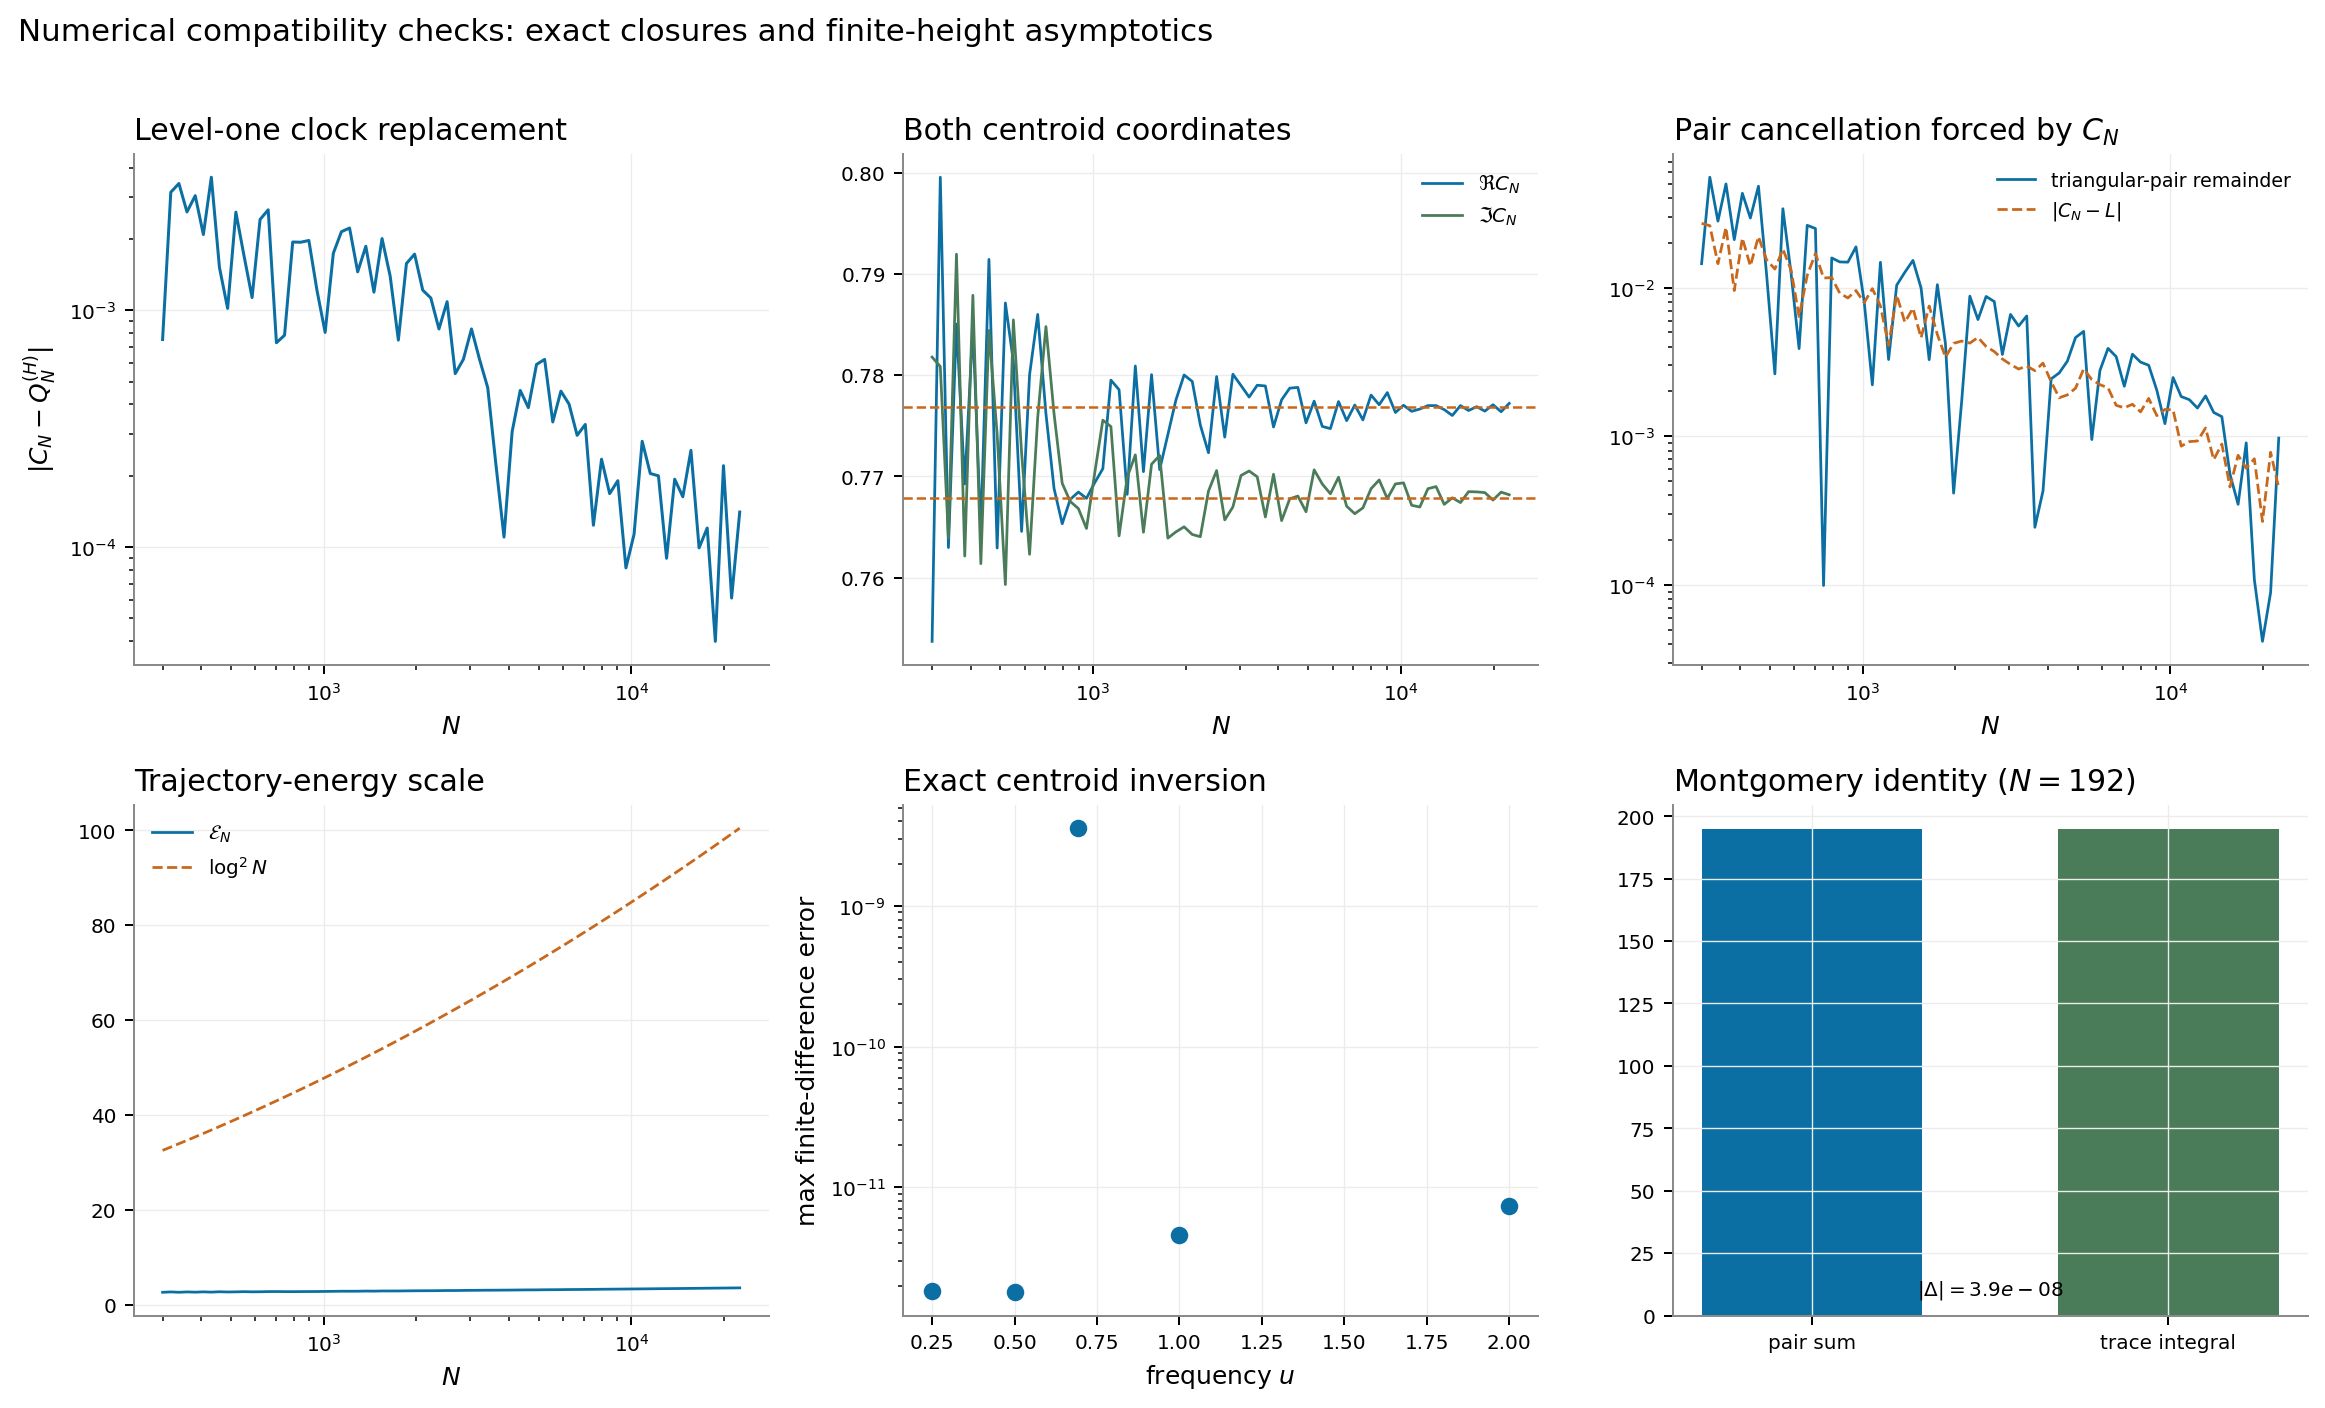
\includegraphics[width=0.99\textwidth]{core_theorem_compatibility.png}
\caption{Inline compatibility checks for Level one, the two centroid
coordinates, both pair identities, exact centroid inversion, and the
Montgomery integral identity.  Algebraic statements are assessed by closure
error; asymptotic statements by their finite-height remainder.}
\label{fig:core_checks}
\end{figure}

These identities make the scale distinction precise.  Convergence of one
complex centroid forces strong pair cancellation at one fixed frequency.  The
Montgomery conjecture asks for a locally rescaled continuum of difference
frequencies.

\section{Exact inversion of the centroid family}

Set
\begin{equation}\label{eq:AN_definition}
A_N(u):=NC_N(u)=\sum_{k\leq N}(N-k+1)\ee^{iu\gamma_k},
\qquad A_0(u)=0.
\end{equation}

\begin{theorem}[Centroid inversion]\label{thm:centroid_inversion}
For every $u\in\mathbb R$ and $N\geq1$,
\begin{equation}\label{eq:centroid_inversion}
\boxed{
\Delta A_N(u)=S_N(u),
\qquad
\Delta^2A_N(u)=\ee^{iu\gamma_N}.}
\end{equation}
Hence
\begin{equation}\label{eq:pair_square}
|\Delta A_N(u)|^2=\sum_{j,k\leq N}\ee^{iu(\gamma_j-\gamma_k)}.
\end{equation}
If $W\in L^1(\mathbb R)$ and
$\widehat W(x)=\int W(v)\ee^{ivx}\dd v$, then
\begin{equation}\label{eq:smoothed_pair_from_centroid}
\boxed{
\int_{\mathbb R}W(v)|\Delta A_N(u+v)|^2\dd v
=\sum_{j,k\leq N}\ee^{iu(\gamma_j-\gamma_k)}
\widehat W(\gamma_j-\gamma_k).}
\end{equation}
\end{theorem}

\begin{proof}
Subtract $A_{N-1}(u)$ from \eqref{eq:AN_definition}; every old phase loses one
copy and the new phase appears once.  A second difference leaves the endpoint.
This is a finite algebraic operation valid for every real $u$, including
$u=0$, and requires neither distinct zeros nor RH.  Expanding the finite square
gives \eqref{eq:pair_square}.  For \eqref{eq:smoothed_pair_from_centroid},
$|\Delta A_N(u+v)|^2\le N^2$; hence
$|W(v)||\Delta A_N(u+v)|^2$ is integrable because $W\in L^1(\mathbb R)$.
Fubini applies to the finite double sum and the absolutely convergent integral,
and its inner integral is exactly $\widehat W(\gamma_j-\gamma_k)$.
\end{proof}

\begin{numericalcheck}
For all $22{,}491$ ordinates and
$u\in\{0.25,0.5,1,\log2,2\}$, the largest finite-difference closure error lies
between $1.79\times10^{-12}$ and $3.57\times10^{-9}$; the larger value occurs
at the Landau-resonant frequency $\log2$, where intermediate sums are much
larger.  See Figure~\ref{fig:core_checks}.
\end{numericalcheck}

The theorem shows that the full frequency-dependent triangular centroid is a
lossless linear encoding of the zero spectrum.  Pair correlation is its
quadratic frequency transform.

\section{Montgomery's form factor and the proved sine law}

Let
\begin{equation}\label{eq:montgomery_weight}
w(x)=\frac4{4+x^2}
=\int_{\mathbb R}\ee^{-2|v|}\ee^{ivx}\dd v.
\end{equation}
For $T$ which is not a zero ordinate, put $N_T=\mathcal N(T)$ and
\begin{equation}\label{eq:centroid_form_factor}
\mathfrak F_T^C(\alpha)
:=\left(\frac{T}{2\pi}\log T\right)^{-1}
\int_{\mathbb R}\ee^{-2|v|}
|\Delta A_{N_T}(\alpha\log T+v)|^2\dd v.
\end{equation}

\begin{proposition}[Exact identification with Montgomery's form factor]
\label{prop:Montgomery_identity}
\begin{equation}\label{eq:Montgomery_identity}
\boxed{
\mathfrak F_T^C(\alpha)
=\left(\frac{T}{2\pi}\log T\right)^{-1}
\sum_{0<\gamma,\gamma'\leq T}
T^{i\alpha(\gamma-\gamma')}w(\gamma-\gamma').}
\end{equation}
\end{proposition}

\begin{proof}
The function $W(v)=\ee^{-2|v|}$ is continuous, belongs to $L^1(\mathbb R)$,
and direct integration over the two half-lines gives
$\widehat W(x)=2/(2-ix)+2/(2+ix)=4/(4+x^2)$.  Use
\eqref{eq:smoothed_pair_from_centroid} with $u=\alpha\log T$.  The restriction
that $T$ is not a zero ordinate fixes $N_T$ without a boundary ambiguity; at a
zero height one may use either one-sided limit after specifying the complete
multiplicity block.
\end{proof}

\begin{numericalcheck}
With the first 192 ordinates and $\alpha=0.65$, direct evaluation of the
weighted pair sum gives $194.792615792839$; trapezoidal quadrature of the
smoothed trace integral gives $194.792615832027$.  The discrepancy
$3.92\times10^{-8}$ is the controlled quadrature/truncation error.
\end{numericalcheck}

\begin{theorem}[Montgomery ramp in centroid form]\label{thm:ramp}
Assume RH.  Uniformly in Montgomery's proved range $|\alpha|\leq1$,
\begin{equation}\label{eq:ramp_asymptotic}
\mathfrak F_T^C(\alpha)
=T^{-2|\alpha|}\log T+|\alpha|+o(1).
\end{equation}
In particular, for fixed $0<|\alpha|\leq1$,
\begin{equation}\label{eq:ramp_limit}
\mathfrak F_T^C(\alpha)\longrightarrow|\alpha|,
\end{equation}
including the first plateau point $|\alpha|=1$.
\end{theorem}

\begin{proof}
By Proposition~\ref{prop:Montgomery_identity}, this is exactly Montgomery's
1973 theorem under RH \cite{Montgomery1973}.  The normalization, the weight
$4/(4+x^2)$, the complete multiplicity convention, and the frequency
$T^{i\alpha(\gamma-\gamma')}$ coincide term by term with his form factor; no
additional limiting interchange is made here.  The pole of $\zeta$ and its
trivial zeros enter Montgomery's explicit-formula proof through known smooth
terms and are not members of the displayed nontrivial-zero sum.
\end{proof}

\begin{numericalcheck}
Using all $22{,}491$ ordinates, local scale
$L_T=\log(T/2\pi)=8.065574267$, Montgomery weight, normalized-gap bin width
$0.01$, and lags through 500 gives RMSE $0.054321$ against the finite ramp on
$0.2\le\alpha\le1$.  At $\alpha=1$, $F_T=1.042061$.
\end{numericalcheck}

Use the Fourier convention
$\widehat f(\alpha)=\int f(x)\ee^{-2\pi i\alpha x}\dd x$.

\begin{corollary}[Band-limited sine law]\label{cor:band_sine}
Assume RH.  For every even Schwartz function with
$\supp\widehat f\subset(-1,1)$,
\begin{align}
&\left(\frac{T}{2\pi}\log T\right)^{-1}
\sum_{0<\gamma,\gamma'\leq T}
f\!\left(\frac{\log T}{2\pi}(\gamma-\gamma')\right)
w(\gamma-\gamma')\notag\\
&\hspace{3em}\longrightarrow
f(0)+\int_{\mathbb R}f(x)
\left[1-\left(\frac{\sin\pi x}{\pi x}\right)^2\right]\dd x.
\label{eq:band_sine}
\end{align}
\end{corollary}

\begin{proof}
Because $f$ is Schwartz, both $f$ and $\widehat f$ are integrable and Fourier
inversion holds pointwise.  The compact support
$\supp\widehat f\subset(-1,1)$ restricts the integral to the range where
Theorem~\ref{thm:ramp} is uniform.  Multiplication by $\widehat f$ supplies an
integrable majorant, so the uniform $o(1)$ may be integrated.  The diagonal
$\gamma=\gamma'$ gives $f(0)$.  With the stated Fourier convention,
$\widehat{(\sin\pi x/(\pi x))^2}(\alpha)=(1-|\alpha|)_+$; hence the
off-diagonal transform $|\alpha|$ on $(-1,1)$ is the Fourier dual of
$1-(\sin\pi x/(\pi x))^2$.  Boundary values at $\alpha=\pm1$ have measure zero
in the inversion integral.
\end{proof}

\begin{numericalcheck}
RVM unfolding of the same table, with positive gaps through lag 16, gives
RMSE $0.0362$ against
$1-(\sin\pi s/(\pi s))^2$ on $0.2\le s\le6$.  Applying the same Hann gap
window to data and reference gives Fourier-dual RMSE $0.0410$ on
$0.1\le\alpha\le1.8$; see Figure~\ref{fig:residual_sine}.
\end{numericalcheck}

Thus a sine law has already been obtained from the centroid under RH: its test
functions are exactly those whose Fourier transform lies in the proved ramp.
The unrestricted law is equivalent to the plateau
\begin{equation}\label{eq:plateau_goal}
\mathfrak F_T^C(\alpha)\longrightarrow1,
\qquad |\alpha|>1.
\end{equation}

\section{Exact RVM unfolding and the residual plateau}

Define the smooth clock
\begin{equation}\label{eq:Mclock}
M(t)=\frac{t}{2\pi}\log\frac{t}{2\pi\ee}+\frac78
\end{equation}
and the exact unfolded residual
\begin{equation}\label{eq:eta}
x_k=M(\gamma_k),
\qquad
\eta_k=x_k-\left(k-\frac12\right).
\end{equation}

\begin{theorem}[Exact residual representation of every pair]
\label{thm:residual_pair}
For all $k,h\geq1$,
\begin{equation}\label{eq:residual_pair}
\boxed{x_{k+h}-x_k=h+\eta_{k+h}-\eta_k.}
\end{equation}
If $r_k=k-\frac12-H(\gamma_k)$ is the ordinal counting defect, then
\begin{equation}\label{eq:eta_rank}
\eta_k=M(\gamma_k)-H(\gamma_k)-r_k=-r_k+O(\gamma_k^{-1}).
\end{equation}
\end{theorem}

\begin{proof}
All quantities are real and finite because $\gamma_k>0$ lies in the domain of
$M$.  Subtract the two definitions in \eqref{eq:eta}; no limiting operation is
present.  Stirling's expansion of $\Log\Gamma$ on the vertical line
$1/4+it/2$, whose distance from the poles of $\Gamma$ is positive, gives
$H(t)-M(t)=1/(48\pi t)+O(t^{-3})$.  Substitution of
$r_k=k-1/2-H(\gamma_k)$ proves \eqref{eq:eta_rank}.  The estimate is uniform
for $k\to\infty$ and is unaffected by repeated ordinates.
\end{proof}

\begin{numericalcheck}
For lags $1\le h\le16$ and all admissible pairs in the table, direct and
residual reconstructions of the unfolded gap agree with maximum floating-point
error $0.000\times10^0$.  After discarding the first 1,200 slots,
$\operatorname{sd}(\eta_k)=0.299245$.
\end{numericalcheck}

For a block $K+1,\ldots,K+H$ define
\begin{equation}\label{eq:unfolded_form_factor}
F_{K,H}^{\rm unf}(\alpha)
=\frac1H\left|\sum_{r=1}^{H}\ee^{2\pi i\alpha x_{K+r}}\right|^2
\end{equation}
and
\begin{equation}\label{eq:Rcov}
R_{K,H}(h;\alpha)
=\frac1{H-h}\sum_{r=1}^{H-h}
\ee^{2\pi i\alpha(\eta_{K+r+h}-\eta_{K+r})}.
\end{equation}
Then
\begin{equation}\label{eq:residual_form_factor}
\boxed{
F_{K,H}^{\rm unf}(\alpha)
=1+2\Re\sum_{h=1}^{H-1}
\left(1-\frac hH\right)\ee^{2\pi i\alpha h}R_{K,H}(h;\alpha).}
\end{equation}
The diagonal is the exact $1$.  Therefore the full content of the plateau is
the vanishing of the displayed off-diagonal sum.

Equivalently, define the positive residual pair measure
\begin{equation}\label{eq:residual_measure}
\mu_{K,H}^{+}
=\frac1H\sum_{r=1}^{H-1}\sum_{h=1}^{H-r}
\delta_{h+\eta_{K+r+h}-\eta_{K+r}}.
\end{equation}
In the bulk regime $K\to\infty$, $H\to\infty$, with compactly supported test
functions in the separation variable, the RVM-unfolded pair conjecture is
\begin{equation}\label{eq:residual_sine}
\boxed{
\mu_{K,H}^{+}\ \stackrel{\rm vague}{\Longrightarrow}
\left[1-\left(\frac{\sin\pi s}{\pi s}\right)^2\right]\dd s.}
\end{equation}
The arrow means vague convergence against $C_c(0,\infty)$ tests.  This
topology is required because the total mass over the unbounded separation
axis grows with $H$.  Replacing the local $M$ scale by the constant
$\log T/(2\pi)$ scale is an asymptotically equivalent, but not finite-$T$
identical, version of Montgomery's global formulation.

At an integer $m\ne0$,
\begin{equation}\label{eq:integer_mode}
\ee^{2\pi imx_k}=(-1)^m\ee^{2\pi im\eta_k};
\end{equation}
the lattice carrier is constant and the cancellation is purely residual.  This
identity explains both the strength of the required cancellation and the need
for the same smoothing used in Montgomery's form factor: a raw finite trace
can retain a narrow coherent spike even when the local pair density follows
the sine law.

\section{The Lambert carrier: closed saddle spectrum and an exact counterexample}

Let $\tau_k$ be defined by
\begin{equation}\label{eq:tau}
M(\tau_k)=k-\frac12,
\qquad
\tau_k=\frac{2\pi(k-11/8)}{W_0((k-11/8)/\ee)}.
\end{equation}
The inverse is explicit and
\begin{equation}\label{eq:tau_derivatives}
M'(t)=\frac1{2\pi}\log\frac{t}{2\pi},
\qquad
\tau'(x)=\frac{2\pi}{\log(\tau(x)/2\pi)}.
\end{equation}

\subsection{Closed archimedean saddle spectrum}

Consider the carrier sum
\begin{equation}\label{eq:carrier}
S_M(t;N)=\sum_{k\leq N}\ee^{it\tau_k},
\qquad T=\tau_N,
\qquad t=\alpha\log(T/2\pi).
\end{equation}

\begin{theorem}[Localized archimedean saddle spectrum]\label{thm:saddles}
Let $\tau(x)$ be the inverse of $M(\tau)=x-1/2$ and insert a
$C_c^\infty$ cutoff in the open ordinal interval before applying Poisson
summation.  The $n$th positive Fourier mode has a stationary point exactly at
\begin{equation}\label{eq:saddle_location}
\boxed{\tau_n^*=2\pi\ee^{t/n}}
\end{equation}
whenever this point lies in the support.  If the cutoff is one near the point
and the point stays away from the support boundary, its leading contribution
as $t\to\infty$ is
\begin{equation}\label{eq:saddle_contribution}
\boxed{
\frac{t\ee^{t/(2n)}}{n^{3/2}}
\exp\!\left(i\left[2\pi n\ee^{t/n}-\frac{11\pi n}{4}-\frac\pi4\right]\right).}
\end{equation}
For fixed nonintegral $\alpha>0$, the leading admissible saddle is
$n_0=\lceil\alpha\rceil$, and
\begin{equation}\label{eq:carrier_normalized}
\frac{\textup{magnitude of the }n_0\textup{ saddle}}{\sqrt N}
\asymp
\sqrt{\log(T/2\pi)}
\left(\frac{T}{2\pi}\right)^{\alpha/(2n_0)-1/2}
\longrightarrow0.
\end{equation}
At an integer $\alpha=m$, the leading saddle reaches the upper endpoint and
the corresponding one-sided endpoint stationary-phase term has
root-logarithmic size relative to $\sqrt N$.  It is a boundary theorem, not a
substitution of $\alpha=m$ into the interior formula.
\end{theorem}

\begin{proof}
On $\tau>2\pi$, $M$ is $C^\infty$, has positive derivative, and maps
bijectively onto $(-1/8,\infty)$.  The inverse-function theorem makes
$\tau(x)$ $C^\infty$.  The $W_0$ representation is real on the arguments in
\eqref{eq:tau}; none is its branch point $-1/\ee$ or its zero.  Poisson
summation is therefore applied to a compactly supported $C^\infty$ function,
so the Fourier series and every integration by parts used below are justified.
The phase of mode $n$ is
\[
\Phi_n(x)=t\tau(x)-2\pi nx.
\]
Since $\tau'(x)=2\pi/\log(\tau/2\pi)$, the stationary equation
$\Phi_n'(x)=0$ is $\log(\tau/2\pi)=t/n$, proving
\eqref{eq:saddle_location}.  Moreover,
\[
\tau''(x)=-\frac{4\pi^2}{\tau\log^3(\tau/2\pi)},
\qquad
|\Phi_n''(x_n)|=\frac{4\pi^2n^3}{\tau_n^*t^2}.
\]
At the critical point $\Phi_n''<0$ and is nonzero.  The amplitude is smooth and
equals one nearby, so the one-dimensional stationary-phase factor
$\sqrt{2\pi/|\Phi_n''(x_n)|}$ is exactly
$t\ee^{t/(2n)}n^{-3/2}$.  Substitution of
$x_n=M(\tau_n^*)+1/2$ gives the phase in
\eqref{eq:saddle_contribution}.  The zero and negative Fourier modes have no
stationary point because $t\tau'(x)>0$; repeated integration by parts controls
them away from the cutoff boundary.  The condition $\tau_n^*\leq T$ is
$n\geq\alpha$; away from integer endpoints, the first admissible mode is
$n_0=\lceil\alpha\rceil$ and is the largest localized saddle contribution.
Finally
$N\sim(T/2\pi)\log(T/2\pi)$, giving
\eqref{eq:carrier_normalized}.  At $\alpha=m$, the $m$th critical point lies at
$T$ and the one-sided stationary-phase theorem gives the asserted scale.
Compact support removes improper endpoints, and no pole or zero of an analytic
factor is crossed.
\end{proof}

\begin{numericalcheck}
On the archived $2{,}001{,}052$-level RVM binary, the median ratio of the
measured carrier amplitude to the leading localized saddle amplitude is
$0.982468$ away from integer endpoints; the RMS relative discrepancy is
$0.113034$.  Representative ratios range from $0.8269$ to $1.0550$.
\end{numericalcheck}

\begin{figure}[htbp]
\centering
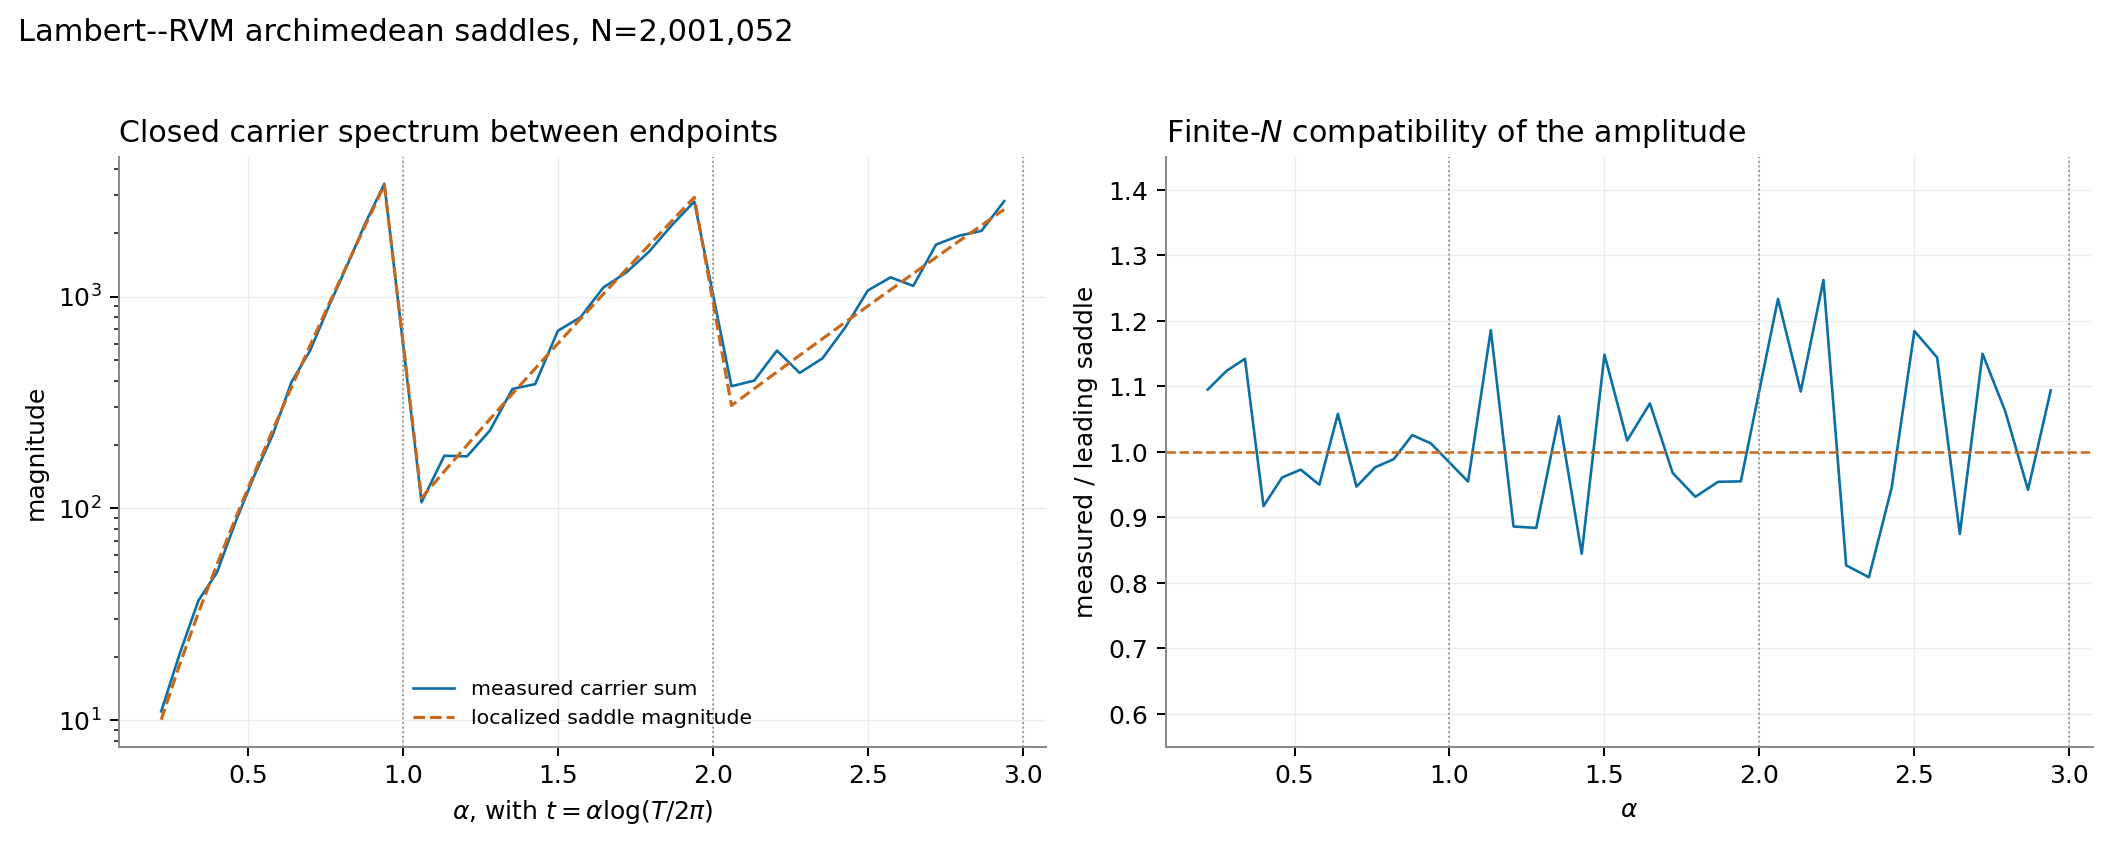
\includegraphics[width=0.98\textwidth]{carrier_saddle_validation.png}
\caption{Closed archimedean saddle spectrum for the Lambert--RVM carrier.
Dashed curves use the stationary location and leading amplitude; the vertical
boundaries are where an interior saddle becomes an endpoint saddle.}
\label{fig:carrier_saddles}
\end{figure}

\subsection{Centroid convergence does not imply sine-kernel pairs}

Define the Lambert carrier centroid
\begin{equation}\label{eq:carrier_centroid}
C_N^M=\sum_{k\leq N}\left(1-\frac{k-1}{N}\right)\ee^{i\tau_k}.
\end{equation}

Put $g_k=\tau_{k+1}-\tau_k$, $v_k=\ee^{i\tau_k}$, and
$d_k=(\ee^{ig_k}-1)^{-1}$.  Since $g_k\downarrow0$ and $g_k<2\pi$ after a
finite initial segment, the denominator never vanishes there; the finite
initial segment is checked directly.

\begin{lemma}[Clock and phase-sum bounds]\label{lem:carrier_bounds}
As $k\to\infty$,
\[
\tau_k\sim\frac{2\pi k}{\log k},\quad
g_k\sim\frac{2\pi}{\log k},\quad
d_k=O(\log k),\quad \Delta d_k=O(k^{-1}),\quad
\Delta^2d_k=O(k^{-2}),
\]
and $\sum_{k\le N}v_k=O(\log N)$.
\end{lemma}

\begin{proof}
The inverse-function identities
$\tau'(x)=1/M'(\tau(x))$ and
$\tau''(x)=-M''(\tau(x))/M'(\tau(x))^3$, together with
$M'(t)=(2\pi)^{-1}\log(t/2\pi)$ and $M''(t)=(2\pi t)^{-1}$, give the first two
asymptotics and the derivative bounds.  The Laurent expansion
$(\ee^{iz}-1)^{-1}=-i/z-1/2+O(z)$ is valid for $0<|z|<2\pi$; differentiating
the smooth interpolation and applying the mean-value theorem gives the two
difference estimates.  Finally $\tau'(x)>0$ is monotone and, on each large
interval $[J,N]$, its distance from $2\pi\mathbb Z$ is bounded below by a
constant multiple of $1/\log N$.  The Kusmin--Landau first-derivative estimate
therefore gives $O(\log N)$; finitely many early terms change only the constant.
\end{proof}

\begin{theorem}[Lambert centroid convergence]\label{thm:carrier_centroid}
The sequence $C_N^M$ converges unconditionally, and
\begin{equation}\label{eq:carrier_rate}
C_N^M=C_\infty^M+O\!\left(\frac{\log^2N}{N}\right).
\end{equation}
\end{theorem}

\begin{proof}
The exact identity
\[
\ee^{i\tau_k}=d_k(\ee^{i\tau_{k+1}}-\ee^{i\tau_k}).
\]
holds because its right side is
$d_kv_k(\ee^{ig_k}-1)=v_k$.  Summing it gives
\[
\sum_{k\le N}v_k=d_Nv_{N+1}-d_1v_1
-\sum_{k=1}^{N-1}(d_{k+1}-d_k)v_{k+1}.
\]
Let $q_k=\Delta d_k$.  Lemma~\ref{lem:carrier_bounds} gives
$q_k=O(k^{-1})$, $\Delta q_k=O(k^{-2})$, and phase partial sums
$O(\log k)$.  Discrete Abel summation, whose finite identity has no convergence
assumption, then gives
\[
\sum_{k\ge J}q_kv_{k+1}=O(\log J/J).
\]
Thus the series
$-d_1v_1-\sum_{k\ge1}q_kv_{k+1}$ converges conditionally.

Averaging the finite endpoint identity from $1$ through $N$ gives exactly
\[
C_N^M=-d_1v_1+\frac1N\sum_{k=1}^Nd_kv_{k+1}
-\sum_{k=1}^{N-1}\left(1-\frac{k}{N}\right)q_kv_{k+1}.
\]
A further Abel summation with $d_k=O(\log k)$ and the phase-sum bound yields
\[
\frac1N\sum_{k\le N}d_kv_{k+1}=O(\log^2N/N).
\]
The infinite-series tail is $O(\log N/N)$, and Abel summation applied to
$N^{-1}\sum_{k<N}kq_kv_{k+1}$ gives the same order.  Adding the three finite
remainders proves \eqref{eq:carrier_rate}.  Every denominator was shown
nonzero above, and all limiting series have now been supplied with a tail
bound.
\end{proof}

\begin{numericalcheck}
For the $2{,}001{,}052$-level clock,
$C_N^M=0.041570229566+1.757541724624i$.  Over 64 doubling pairs,
$|C_{2N}^M-C_N^M|N/\log^2N$ has mean $0.0182816$ and standard deviation
$0.0086594$, compatible with \eqref{eq:carrier_rate} without estimating the
unknown limit from the last point.
\end{numericalcheck}

\begin{corollary}[Exact counterexample to centroid $\Rightarrow$ pairs]
\label{cor:counterexample}
The centroid $C_N^M$ converges, but its unfolded pair measure is
\begin{equation}\label{eq:lattice_pair_measure}
\frac1H\sum_{r=1}^{H-1}\sum_{h=1}^{H-r}
\delta_{M(\tau_{K+r+h})-M(\tau_{K+r})}
=\frac1H\sum_{r=1}^{H-1}\sum_{h=1}^{H-r}\delta_h,
\end{equation}
a finite Dirac comb.  It cannot converge to the continuous sine-kernel density.
\end{corollary}

\begin{proof}
Equation~\eqref{eq:tau} gives
$M(\tau_{k+h})-M(\tau_k)=(k+h-1/2)-(k-1/2)=h$ exactly.  Hence every atom is
supported on the closed discrete set $\mathbb N$.  Choose a nonnegative
$\phi\in C_c(0,\infty)$ supported in a small interval containing no integer
and with positive integral against the sine density.  Every RVM pair measure
integrates $\phi$ to zero, whereas the proposed continuous limit integrates it
positively.  Vague convergence to the sine density is therefore impossible.
\end{proof}

\begin{numericalcheck}
The generated binary satisfies the defining clock equation with maximum
extended-precision residual $4.55\times10^{-13}$.  Its unfolded pair locations
are therefore integer to construction precision; Figure~\ref{fig:rvm_counter}
shows the Dirac comb beside the continuous sine density.
\end{numericalcheck}

\begin{figure}[htbp]
\centering
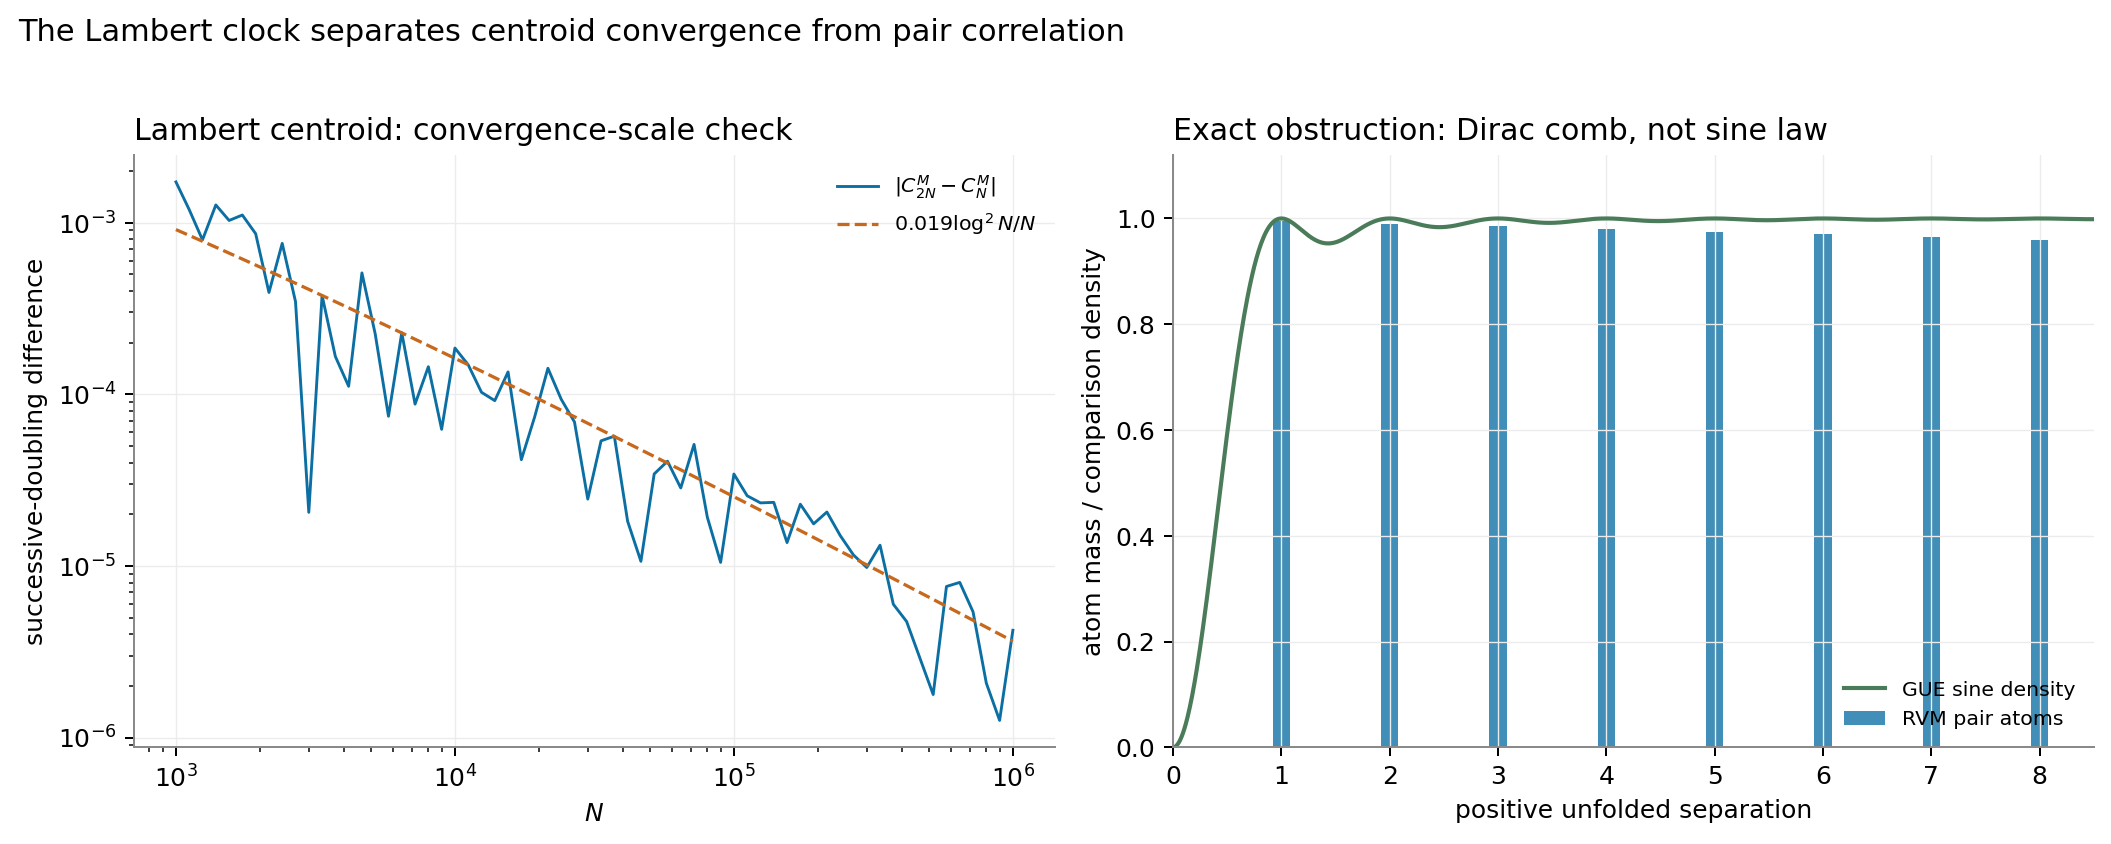
\includegraphics[width=0.98\textwidth]{rvm_counterexample_validation.png}
\caption{Exact counterexample.  Left: successive-doubling centroid differences
on the $\log^2N/N$ scale.  Right: the unfolded RVM pair measure is supported on
integer atoms and cannot approach the continuous sine law.}
\label{fig:rvm_counter}
\end{figure}

This counterexample separates the two mechanisms cleanly.  An order-one
centroid limit is a fixed-frequency linear cancellation.  The sine law is a
scale-dependent quadratic statement about all residual increments.

\section{Where the remaining pair problem enters the centroid proof}

For real $a$ define
\begin{equation}\label{eq:Ja}
\mathcal J_a(T)=\int_{0^-}^{T}\ee^{iat}S_*(t)\,\dd\mathcal N(t).
\end{equation}
The proof of Theorem~\ref{thm:level_one} works at every finite frequency and
gives
\begin{equation}\label{eq:Ja_decomp}
\boxed{
\mathcal J_a(T)
=\frac12\ee^{iaT}S(T)^2
-\frac{ia}{2}\int_0^T\ee^{iat}S(t)^2\dd t
+\int_0^T\ee^{iat}H'(t)S(t)\dd t+O(1).}
\end{equation}
At $a=\alpha\log T$, normalization by $\mathcal N(T)\asymp T\log T$ leaves the
specific quadratic target
\begin{equation}\label{eq:twisted_S2_goal}
\boxed{
\frac1T\int_0^T\ee^{i\alpha\log T\,t}S(t)^2\dd t\longrightarrow0.}
\end{equation}

Let $\dd D=\dd\mathcal N-\dd H$ and $\Sigma(t)=D((0,t])$.  Stieltjes--Fubini
shows that the same target is a connected pair transform:
\begin{align}
\int_0^T\ee^{iat}\Sigma(t)^2\dd t
&=\iint_{(0,T]^2}K_{a,T}(u,v)\,\dd D(u)\dd D(v),\label{eq:connected_pair_kernel}\\
K_{a,T}(u,v)
&=\frac{\ee^{iaT}-\ee^{ia\max(u,v)}}{ia}.
\end{align}
Thus pair correlations are already present in the proof of the centroid; fixed
frequency suppresses them through Selberg's untwisted second moment, whereas
Montgomery frequency exposes their oscillatory transform.

\subsection{The truncated prime-polynomial part can be closed}

Let
\begin{equation}\label{eq:PY}
P_Y(t)=-\frac1\pi\sum_{n\leq Y}
\frac{\Lambda(n)}{\sqrt n\log n}\sin(t\log n).
\end{equation}

\begin{proposition}[Twisted quadratic cancellation in the prime model]
\label{prop:prime_model}
Fix $0<\alpha<2$ and choose
\begin{equation}\label{eq:theta_range}
\frac\alpha2<\theta<\min(\alpha,1),
\qquad Y=T^\theta,
\qquad a=\alpha\log T.
\end{equation}
Then, for every $\varepsilon>0$,
\begin{equation}\label{eq:prime_model_bound}
\int_0^T\ee^{iat}P_Y(t)^2\dd t
\ll_\varepsilon
T^{1-\alpha/2+\varepsilon}
+T^{\alpha/2+\varepsilon}
+T^{\theta+\varepsilon}
=o(T).
\end{equation}
\end{proposition}

\begin{proof}
The polynomial is finite, hence continuous and entire in $t$; its square may
be expanded and integrated term by term on the compact interval $[0,T]$
without a convergence theorem.  Write
$b_n=\Lambda(n)/(\sqrt n\log n)$ for $n\ge2$.  The identity
$\sin u\sin v=\tfrac12[\cos(u-v)-\cos(u+v)]$ produces ratio frequencies
$\log(m/n)$ and product frequencies $\log(mn)$.  For every real $\omega$,
\begin{equation}\label{eq:osc_integral_bound}
\left|\int_0^T\ee^{i\omega t}\dd t\right|
\le\min(T,2/|\omega|),
\end{equation}
with the value at $\omega=0$ defined by continuity as $T$.

Since $m/n\leq Y=T^\theta$ and $\theta<\alpha$,
$|a-\log(m/n)|\ge(\alpha-\theta)\log T$; the other signed ratio frequencies
are farther away.  The elementary estimate
$\sum_{n\le Y}|b_n|\ll\sqrt Y$ then bounds the whole ratio branch by
$O(Y/\log T)$, which is $O(T^{\theta+\varepsilon})$.

For the product branch group $q=mn$ and use
\[
\sum_{mn=q}
\frac{\Lambda(m)\Lambda(n)}{\sqrt{mn}\log m\log n}
\ll_\varepsilon q^{-1/2+\varepsilon}.
\]
The divisor bound $d(q)\ll_\varepsilon q^\varepsilon$ proves the displayed
coefficient estimate, including prime powers and repeated factorizations.
With $X=T^\alpha$,
\[
\left|\int_0^T\ee^{it(a-\log q)}\dd t\right|
\leq\min\!\left(T,\frac2{|\log(X/q)|}\right).
\]
For $q\notin[X/2,2X]$, the denominator in
\eqref{eq:osc_integral_bound} is bounded by its logarithmic distance from
$X$; dyadic summation and $q\le Y^2$ give
$O(T^{\theta+\varepsilon})$.  On $[X/2,2X]$ the mean-value theorem for
$\log$ gives $|\log(X/q)|\asymp|X-q|/X$.  The one nearest integer (including
the exact resonance $q=X$ when $X$ is integral) contributes
$O(TX^{-1/2+\varepsilon})$.  Grouping all remaining integers by
$r=|q-X|\ge1$ gives
$O(X^{1/2+\varepsilon}\sum_{r\le X}r^{-1})
=O(X^{1/2+2\varepsilon})$ after renaming $2\varepsilon$ as $\varepsilon$.
Substituting $X=T^\alpha$ proves \eqref{eq:prime_model_bound}.

Finally, the interval in \eqref{eq:theta_range} is nonempty exactly because
$0<\alpha<2$: if $\alpha\le1$, then $\alpha/2<\alpha$; if
$1<\alpha<2$, then $\alpha/2<1$.  Each exponent in
\eqref{eq:prime_model_bound} is $<1$:
$1-\alpha/2<1$, $\alpha/2<1$, and $\theta<1$.  Division by $T$ therefore
gives $o(1)$.
\end{proof}

\begin{numericalcheck}
The finite polynomial was integrated exactly through exponential
antiderivatives, not time discretization.  For
$(\alpha,\theta)=(0.5,0.375),(1,0.75),(1.5,0.875)$ and
$300\le T\le12{,}000$, the observed $|I(T)|/T$ ranges from
$1.97\times10^{-5}$ to $3.57\times10^{-3}$ and remains below $0.0057$ times
the three-term bound shape used in the proof; see
Figure~\ref{fig:prime_model}.
\end{numericalcheck}

\begin{figure}[htbp]
\centering
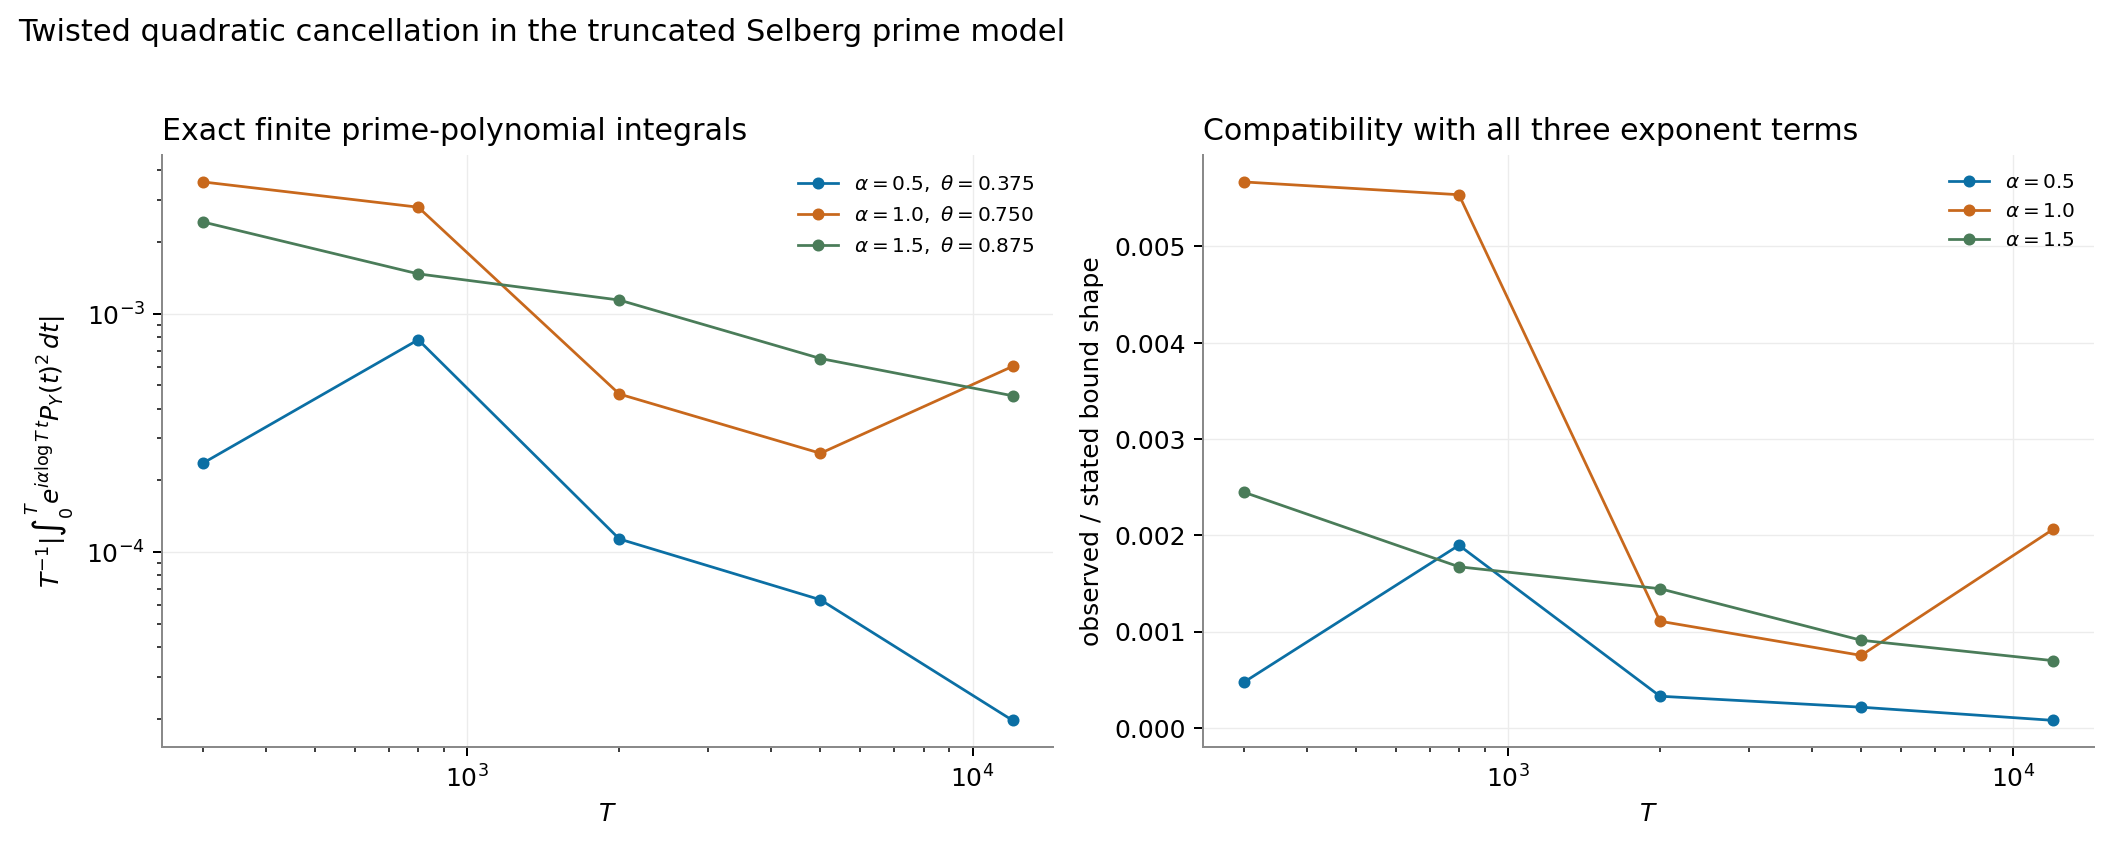
\includegraphics[width=0.98\textwidth]{prime_model_validation.png}
\caption{Exact finite-sum compatibility check for the twisted truncated-prime
proposition.  Every plotted integral is obtained from the closed exponential
antiderivative, including exact product resonances.}
\label{fig:prime_model}
\end{figure}

Write
\begin{equation}\label{eq:Selberg_remainder}
S(t)=P_Y(t)+E_Y(t).
\end{equation}
Proposition~\ref{prop:prime_model} removes the $P_Y^2$ contribution from
\eqref{eq:twisted_S2_goal}.  The transfer to $S^2$ is therefore reduced to
\begin{equation}\label{eq:transfer_target}
\boxed{
\int_0^T\ee^{iat}
\left(2P_Y(t)E_Y(t)+E_Y(t)^2\right)\dd t=o(T).}
\end{equation}
\begin{hypothesis}[Frequency-localized Selberg transfer]\label{hyp:transfer}
For the parameter ranges in which the full plateau is claimed,
\eqref{eq:transfer_target} holds uniformly on compact $\alpha$-intervals.
\end{hypothesis}

This is the isolated analytic lemma left by the centroid route.  It is not a
consequence of Proposition~\ref{prop:prime_model}.  An untwisted
$L^2$ estimate followed by Cauchy--Schwarz discards the oscillation and is too
coarse; the required estimate is a frequency-localized Selberg remainder
bound.  Once \eqref{eq:transfer_target} is available uniformly in a plateau
interval, the quadratic obstruction in the scale-dependent Level-one proof is
removed there.  The exact residual formula \eqref{eq:residual_form_factor}
then identifies the same conclusion as off-diagonal plateau decorrelation.

\begin{numericalcheck}
The connected form factor supplies a finite-data check of the conclusion that
Hypothesis~\ref{hyp:transfer} would imply: on $1\le\alpha\le4$ its
off-diagonal RMS is $0.019680$.  This checks compatibility of the target, not
the unproved uniform remainder estimate itself.
\end{numericalcheck}

\section{Numerical evidence and independent cross-checks}

All computations in this section are reproduced by the Python sources in the
appendices.  The input is an independently generated array of $22{,}491$
ordinates ending at $T=19999.2756\ldots$, exported as raw little-endian
IEEE-754 float64.  The synthetic carrier checks use a second binary containing
$2{,}001{,}052$ Lambert--RVM levels.  Every digest, byte count, command output,
and source is archived.

\begin{center}\small
\begin{longtable}{@{}p{0.31\textwidth}p{0.27\textwidth}p{0.32\textwidth}@{}}
\toprule
Result & Finite check & Observed value\\
\midrule
\endhead
Level-one reduction & $C_N$ versus $Q_N^{(H)}$ & $1.40659\times10^{-4}$\\
Conditional complex limit & two-coordinate error & $4.48101\times10^{-4}$\\
Triangular pair identity & direct $N=512$ closure & $9.66\times10^{-13}$\\
Trajectory pair identity & direct $N=512$ closure & $1.11\times10^{-12}$\\
Centroid inversion & five frequencies & $1.79\times10^{-12}$ to $3.57\times10^{-9}$\\
Montgomery identity & pair sum versus integral & $3.92\times10^{-8}$\\
Montgomery ramp & RMSE, $0.2\le\alpha\le1$ & $0.054321$\\
Residual pair identity & all lags $h\le16$ & zero at float64 resolution\\
Sine pair density & RMSE, $0.2\le s\le6$ & $0.0362$\\
Carrier saddle law & median measured/predicted & $0.982468$\\
Lambert centroid rate & doubling compensation & $0.01828\pm0.00866$\\
Connected plateau & RMS, $1\le\alpha\le4$ & $0.019680$\\
Prime polynomial & max observed/bound shape & $0.0057$\\
\bottomrule
\end{longtable}
\end{center}

\subsection{Residual pair density and sine law}

Unfolding by $M$ gives residual standard deviation $0.299245$.  Reconstructing
all positive gaps through \eqref{eq:residual_pair} with lags through $16$ gives
RMSE $0.0362$ against the sine density on $0.2\leq s\leq6$.  Applying the same
Hann gap window to data and reference gives form-factor RMSE $0.0410$ on
$0.1\leq\alpha\leq1.8$.

\begin{figure}[htbp]
\centering
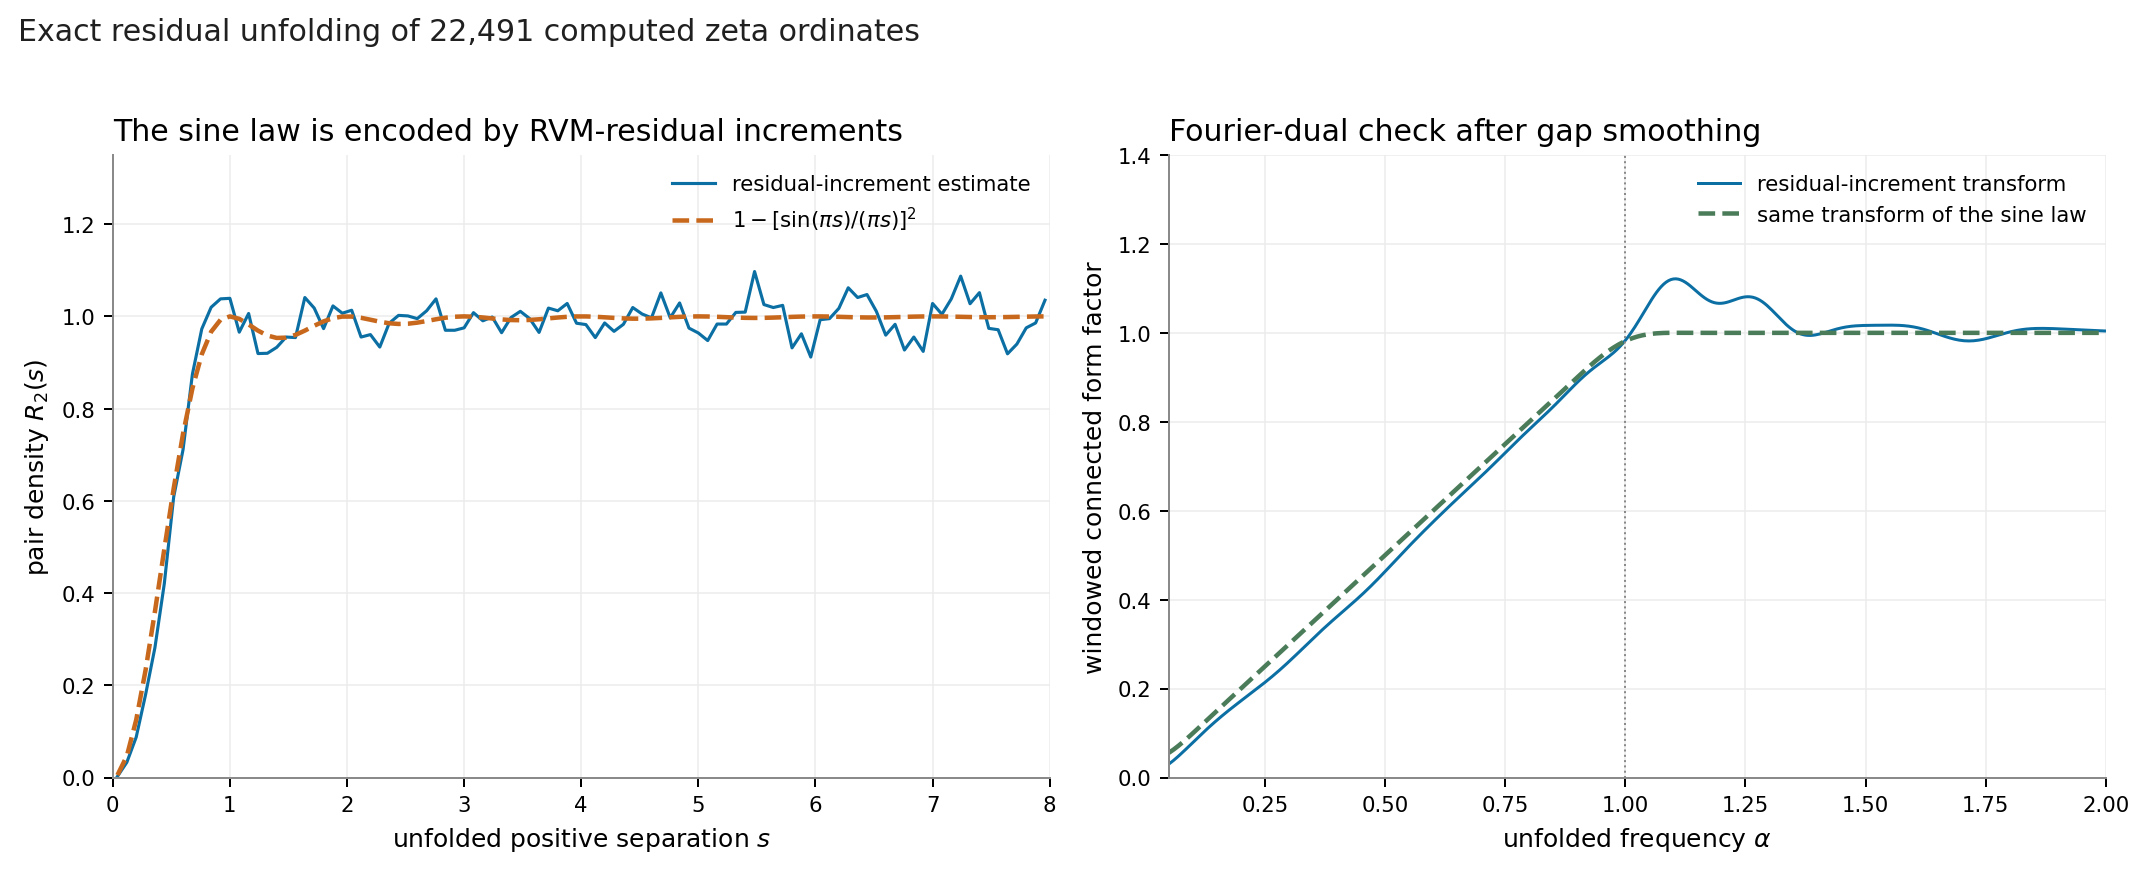
\includegraphics[width=0.98\textwidth]{unfolded_residual_pair_law.png}
\caption{The exact residual identity reconstructs the unfolded pair process.
Left: positive pair density and the sine law.  Right: the Fourier-dual
connected statistic after applying the same compact gap window to data and
reference.}
\label{fig:residual_sine}
\end{figure}

\subsection{The connected form factor}

The form factor is split as
\begin{equation}\label{eq:off_definition}
F_T(\alpha)=1+\Off_T(\alpha),
\end{equation}
where the diagonal is exactly $1$.  The attached computation is reproduced in
English from the same ordinate array.  With the Montgomery weight and ordinal
lags through $500$, the plateau RMS on $1\leq\alpha\leq4$ is $0.01968$, equal
to $0.366\,\log(T/2\pi)/\sqrt N$.

\begin{figure}[htbp]
\centering
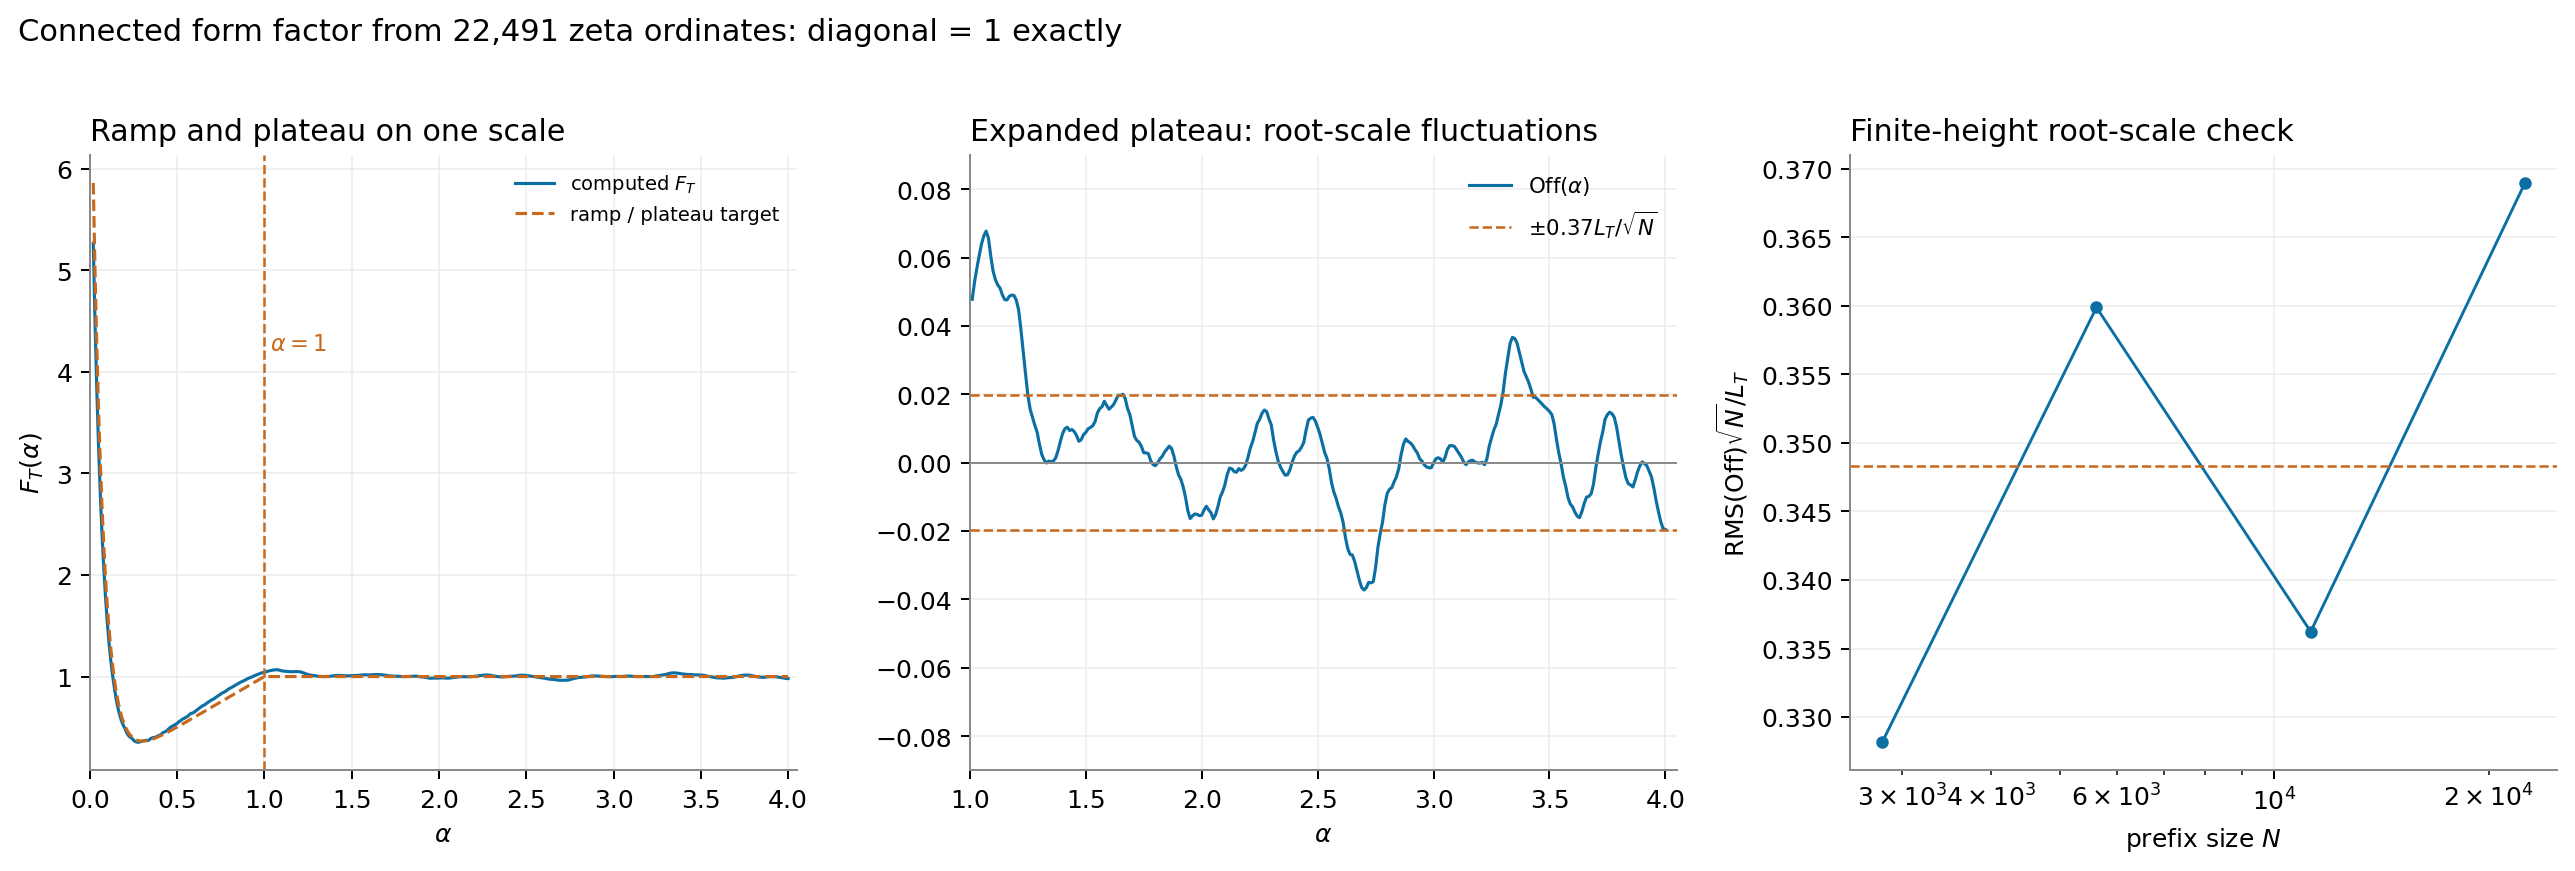
\includegraphics[width=0.98\textwidth]{connected_form_factor.png}
\caption{Connected form factor.  The diagonal contribution is exactly one, so
the plateau conjecture is the disappearance of $\Off_T(\alpha)$.  Left: ramp
and plateau together.  Center: expanded plateau.  Right: prefix scaling of its
RMS.}
\label{fig:connected_form_factor}
\end{figure}

\subsection{Independent \texorpdfstring{$\log N/N$}{log(N)/N} centroid-rate validation}

For $300\leq N\leq22{,}491$, the independent ordinate table gives
\begin{equation}\label{eq:empirical_rate}
\frac{|C_N(1)-L|N}{\log N}
=1.1447\pm0.2589
\end{equation}
over logarithmically spaced cutoffs, with no visible drift.  Extrapolation to
$N=2{,}001{,}052$ predicts $8.3002\times10^{-6}$.  The independent full-table
computation gives $|C_N-Q_N^{(H)}|=8.7162\times10^{-6}$, a ratio $1.0501$ to the
prediction.  These are not identical finite error observables, but their order,
scale, and 90-fold extrapolation agree.

\begin{figure}[htbp]
\centering
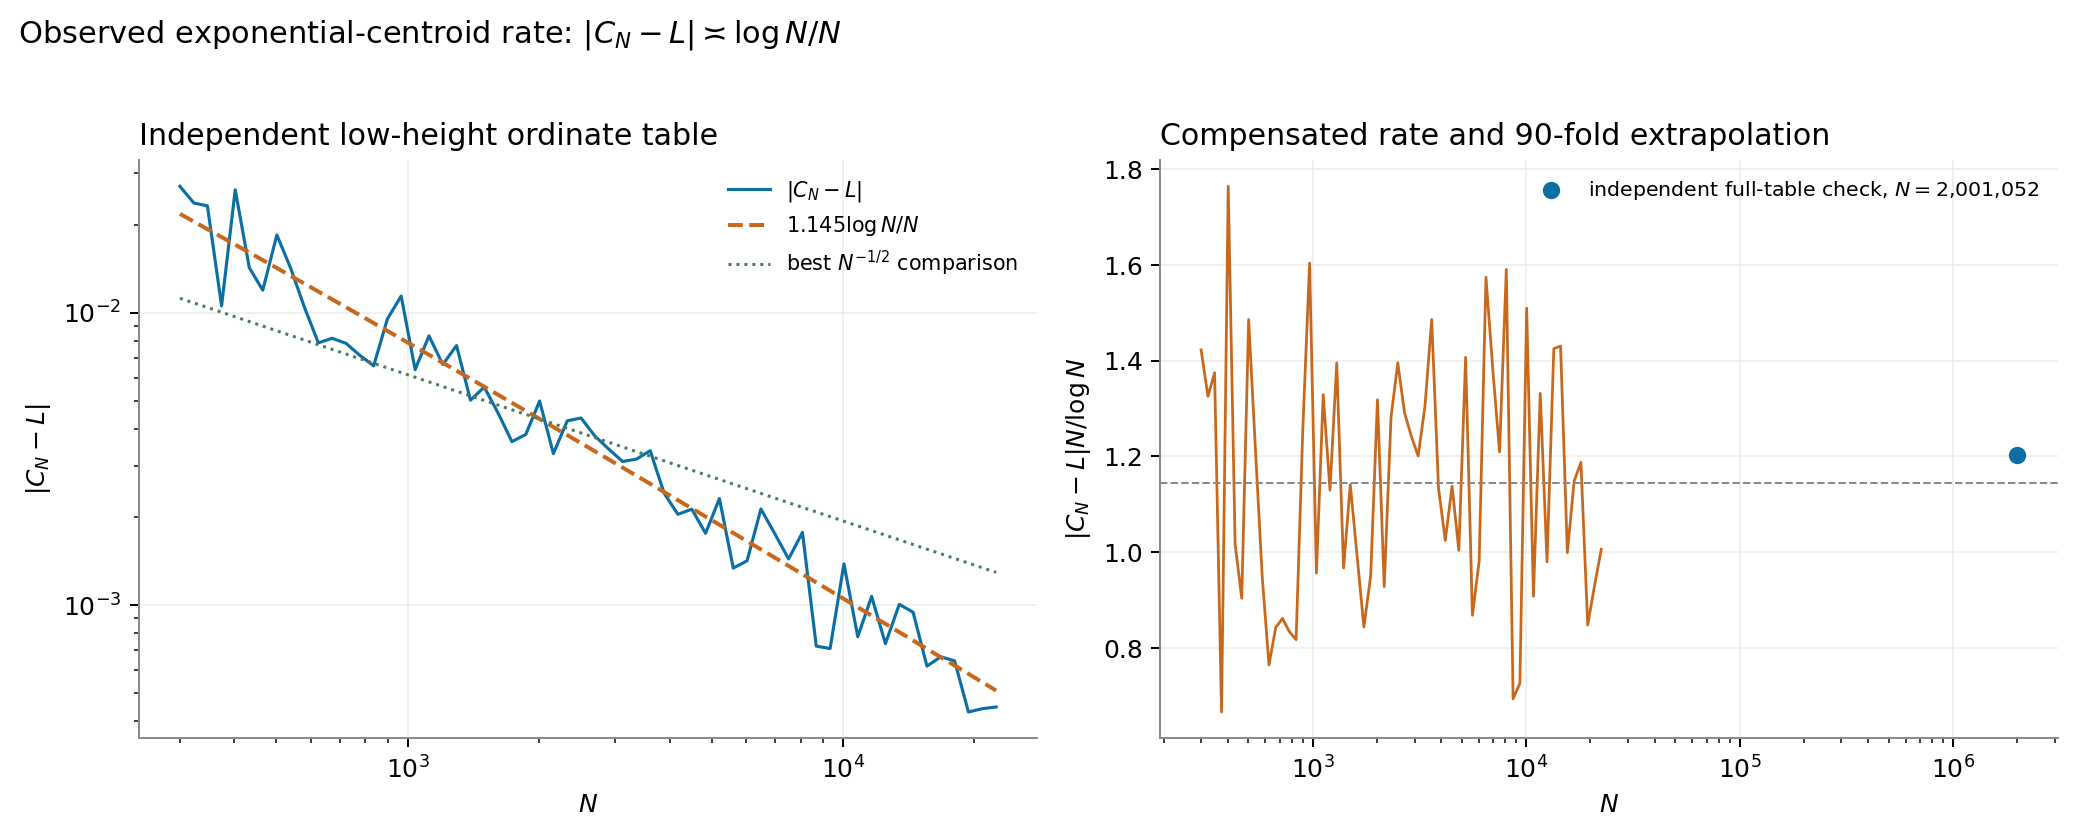
\includegraphics[width=0.96\textwidth]{centroid_rate_validation.png}
\caption{Independent validation of the empirical $\log N/N$ centroid rate.
The right panel includes the full-table check at $N=2{,}001{,}052$.}
\label{fig:centroid_rate}
\end{figure}

\subsection{Same-scale three-dimensional phase clouds}

The following figures use point clouds only: no line joins successive
ordinates.  Within each pair, azimuth, elevation, real limits, imaginary
limits, and ordinal-fraction limits are identical.  The orange cross is the
centroid of the complete cumulative-walk cloud.  Thus morphology is compared
without an automatic rescaling that could hide the size difference.

\begin{figure}[htbp]
\centering
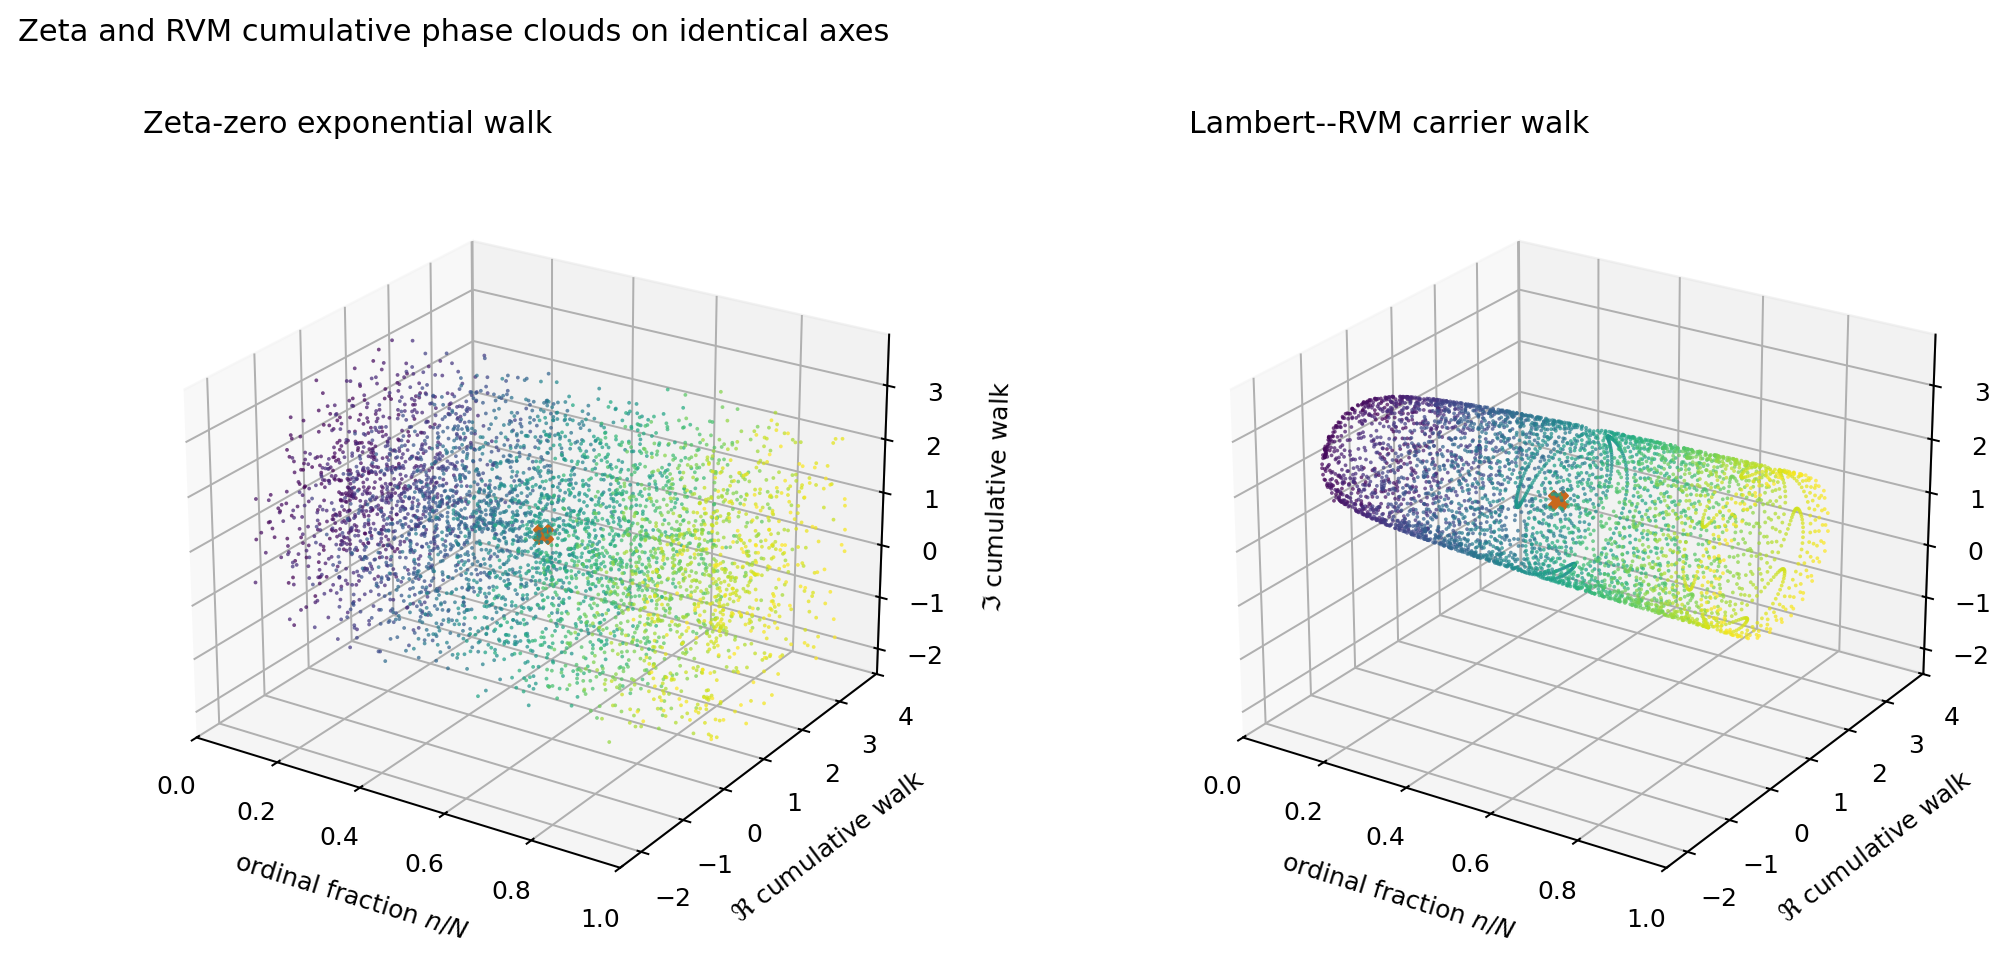
\includegraphics[width=0.99\textwidth]{zeta_rvm_walks_3d_same_scale.png}
\caption{Zeta and Lambert--RVM cumulative exponential walks on identical 3D
axes.  The carrier traces a rigid tube; the true-zero walk fills a visibly
broader phase cloud.}
\label{fig:walks_3d}
\end{figure}

\begin{figure}[htbp]
\centering
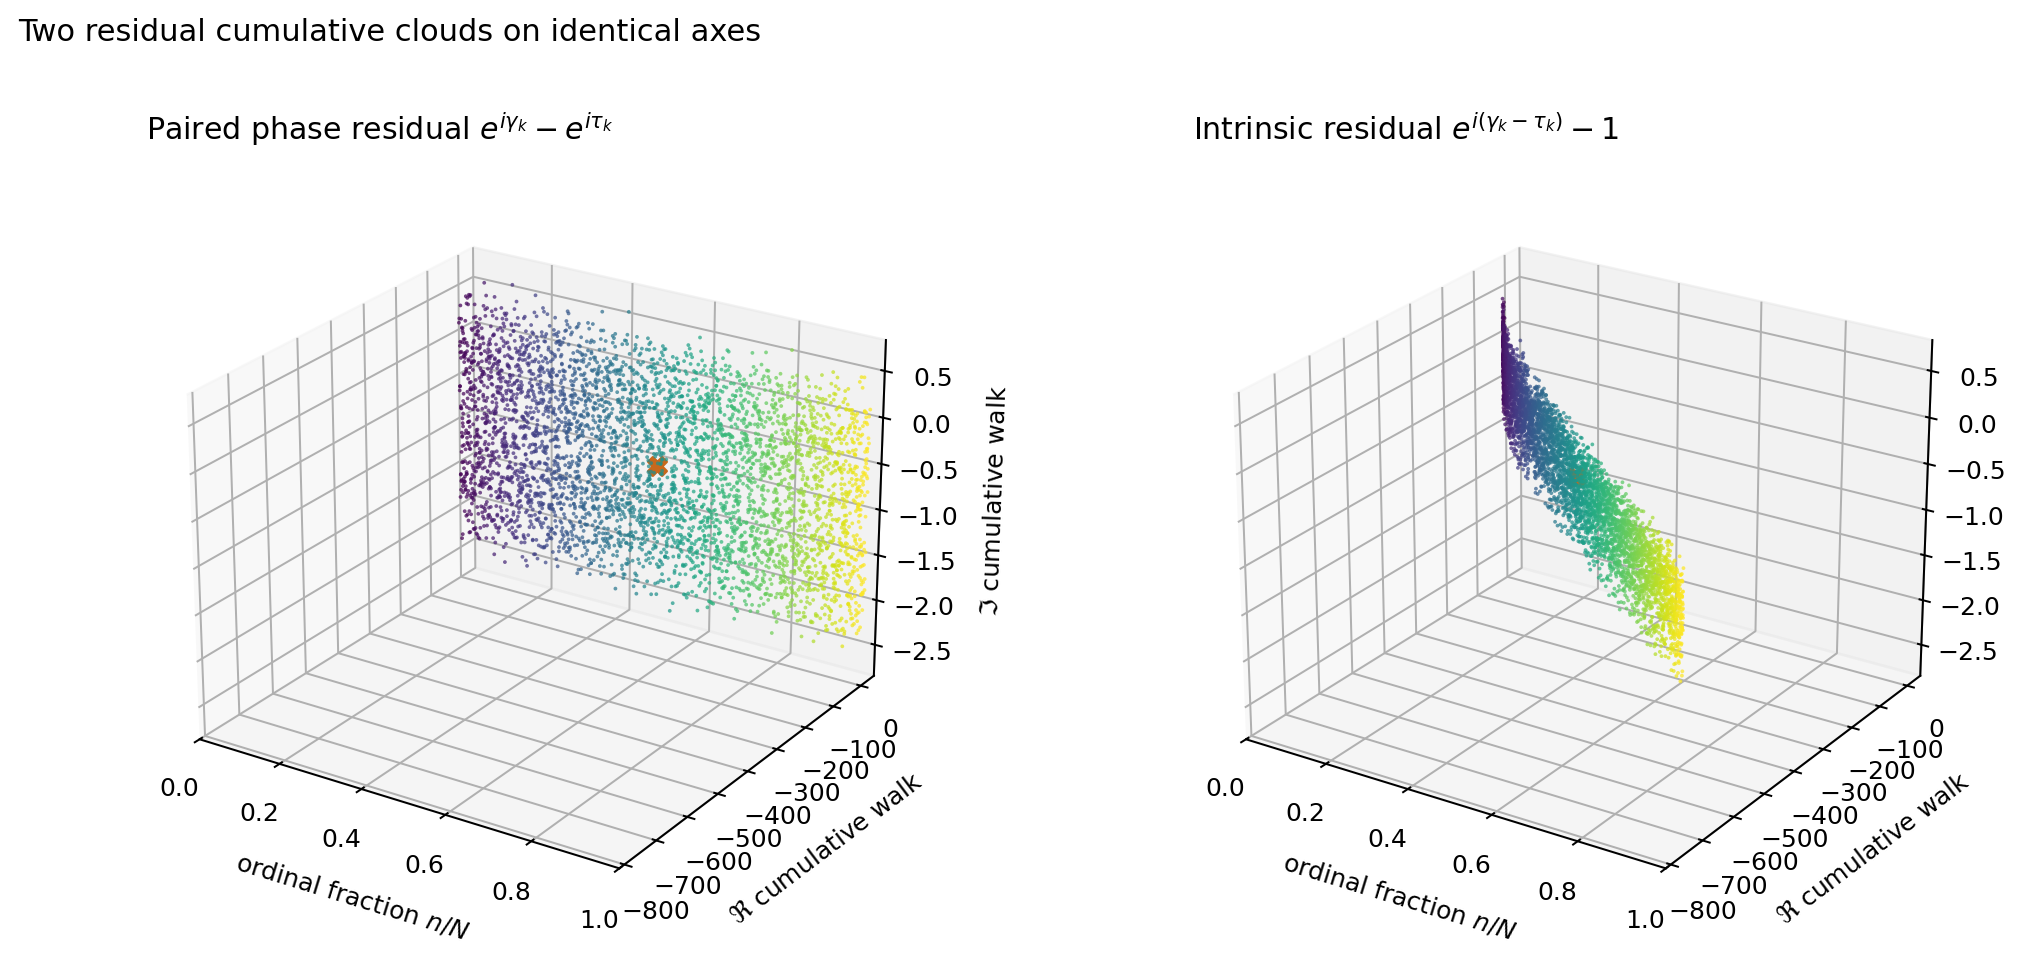
\includegraphics[width=0.99\textwidth]{residual_walks_3d_same_scale.png}
\caption{The two residual cumulative point clouds on identical 3D axes.  Left:
paired phase residual $\ee^{i\gamma_k}-\ee^{i\tau_k}$.  Right: intrinsic
residual $\ee^{i(\gamma_k-\tau_k)}-1$.  The common scale is deliberately
retained even though it compresses the smaller cloud.}
\label{fig:residual_walks_3d}
\end{figure}

\subsection{The supplied form-factor figure}

For provenance, the originally supplied Spanish-language form-factor image is
preserved without alteration in Figure~\ref{fig:supplied_formfactor}; the
English reproduction in Figure~\ref{fig:connected_form_factor} is generated by
the archived Python source and records its numerical parameters.

\begin{figure}[htbp]
\centering
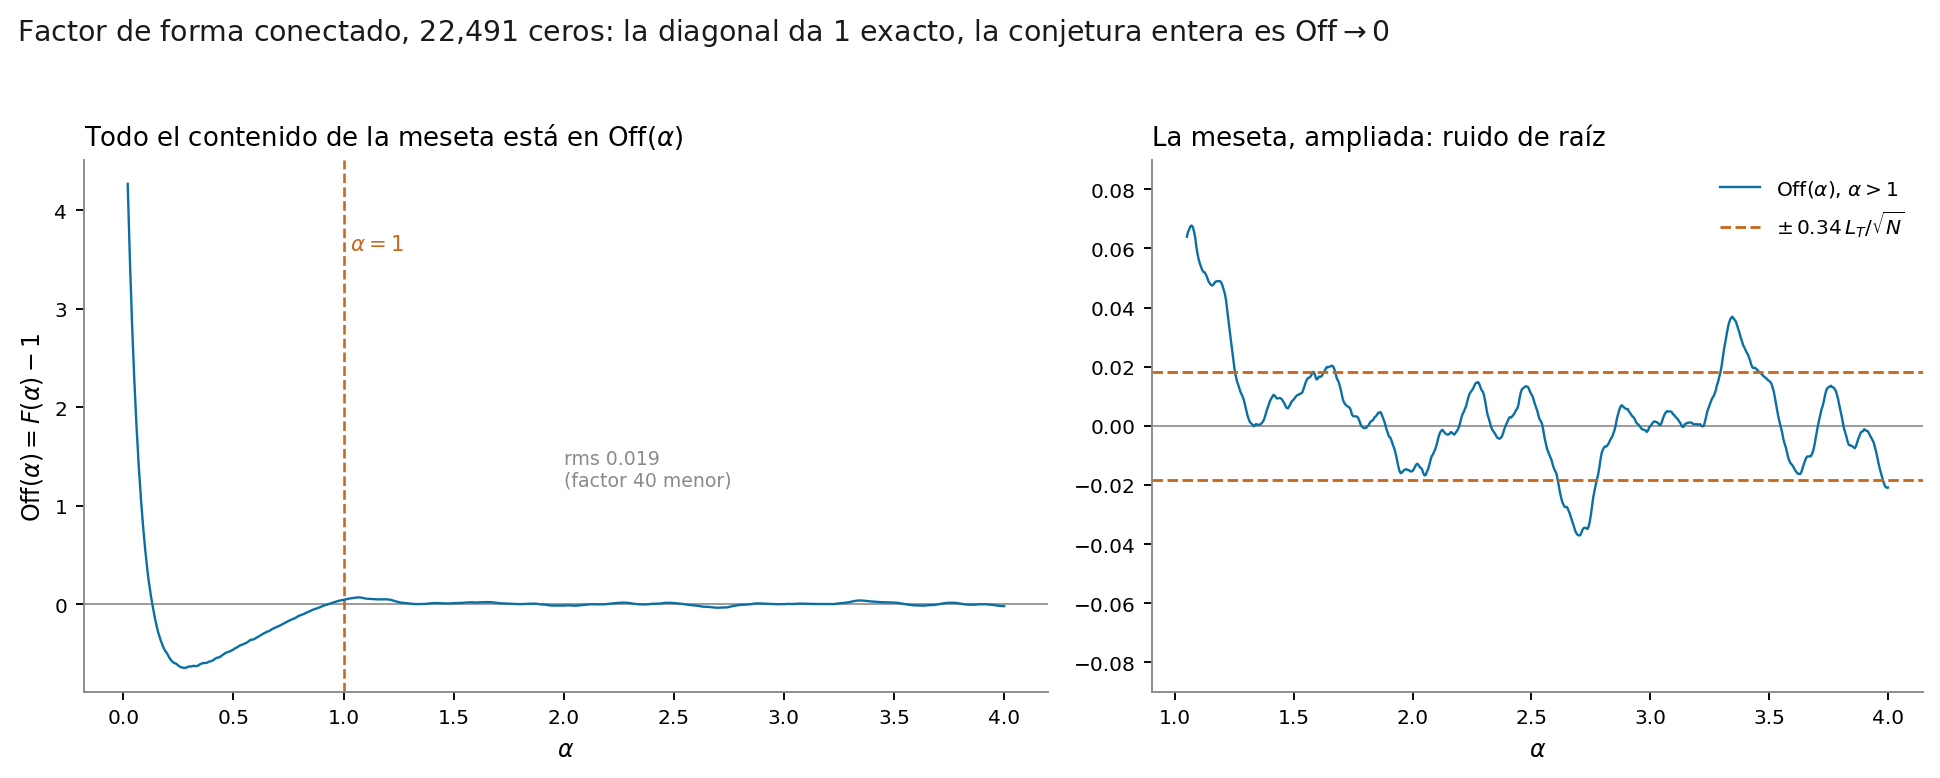
\includegraphics[width=0.98\textwidth]{formfactor_supplied.png}
\caption{Original connected-form-factor figure supplied with the project,
preserved verbatim.}
\label{fig:supplied_formfactor}
\end{figure}

\section{Conclusion}

The exponential centroid supplies more than a geometric statistic.  Its first
ordinal difference is the exponential trace, its second difference recovers
each zero phase, and a smoothed quadratic transform is exactly Montgomery's
form factor.  This proves that a centroid-based route loses no spectral or pair
information.

Three distinct conclusions are now separated rigorously.  First, under RH the
centroid formulation contains Montgomery's proved ramp and hence the
band-limited sine law.  Second, convergence of one centroid forces substantial
fixed-frequency pair cancellation but cannot imply GUE by itself: the Lambert
carrier gives an exact counterexample, with a convergent centroid and a lattice
pair measure.  Third, after exact RVM unfolding, the unrestricted sine law is
equivalent to decorrelation of the increments $\eta_{k+h}-\eta_k$.

The carrier is analytically closed: its Poisson spectrum consists of explicit
archimedean saddles $2\pi\ee^{t/n}$ with amplitude
$t\ee^{t/(2n)}n^{-3/2}$.  The arithmetic is therefore isolated in the true-zero
residual.  On the analytic side, the truncated Selberg prime polynomial already
satisfies the required twisted quadratic cancellation for $0<\alpha<2$.  The
remaining proof target is the frequency-localized transfer
\eqref{eq:transfer_target}.  This is a single, explicit remainder estimate, not
an unspecified appeal to additional cancellation.

\begin{thebibliography}{99}

\bibitem{Montgomery1973}
H.~L.~Montgomery,
\emph{The pair correlation of zeros of the zeta function},
Proc. Sympos. Pure Math. \textbf{24}, AMS, 1973, 181--193.

\bibitem{Titchmarsh}
E.~C.~Titchmarsh, revised by D.~R.~Heath-Brown,
\emph{The Theory of the Riemann Zeta-Function}, 2nd ed.,
Oxford University Press, 1986.

\bibitem{Selberg}
A.~Selberg,
\emph{Contributions to the theory of the Riemann zeta-function},
Arch. Math. Naturvid. \textbf{48} (1946), 89--155.

\bibitem{Gonek}
S.~M.~Gonek,
\emph{An explicit formula of Landau and its applications to the theory of the
zeta-function},
Contemp. Math. \textbf{143} (1993), 395--413.

\bibitem{Landau1912}
E.~Landau,
\emph{Über die Nullstellen der Zetafunktion},
Math. Ann. \textbf{71} (1912), 548--564.

\bibitem{FordZaharescu2005}
K.~Ford and A.~Zaharescu,
\emph{On the distribution of imaginary parts of zeros of the Riemann zeta
function},
J. Reine Angew. Math. \textbf{579} (2005), 145--158.

\end{thebibliography}

\appendix

\section{Shared binary loader}
\lstinputlisting[language=Python]{scripts/data_io.py}

\section{Python source and output: binary export}
\lstinputlisting[language=Python]{scripts/export_binary_data.py}
\lstinputlisting{outputs/export_binary_data_output.txt}

\section{Python source and output: Lambert--RVM binary generation}
\lstinputlisting[language=Python]{scripts/generate_rvm_binary.py}
\lstinputlisting{outputs/generate_rvm_binary_output.txt}

\section{Python source and output: core theorem checks}
\lstinputlisting[language=Python]{scripts/verify_core_theorems.py}
\lstinputlisting{outputs/core_theorem_compatibility_output.txt}

\section{Python source: connected form factor}
\lstinputlisting[language=Python]{scripts/connected_form_factor.py}

\section{Output: connected form factor}
\lstinputlisting{outputs/connected_form_factor_output.txt}

\section{Python source: residual pair law}
\lstinputlisting[language=Python]{scripts/analyze_unfolded_residual_pair_law.py}

\section{Output: residual pair law}
\lstinputlisting{outputs/unfolded_residual_pair_law_output.txt}

\section{Python source: centroid-rate validation}
\lstinputlisting[language=Python]{scripts/centroid_rate_validation.py}

\section{Output: centroid-rate validation}
\lstinputlisting{outputs/centroid_rate_validation_output.txt}

\section{Python source and output: carrier saddle spectrum}
\lstinputlisting[language=Python]{scripts/carrier_saddle_validation.py}
\lstinputlisting{outputs/carrier_saddle_validation_output.txt}

\section{Python source and output: Lambert counterexample}
\lstinputlisting[language=Python]{scripts/rvm_counterexample_validation.py}
\lstinputlisting{outputs/rvm_counterexample_validation_output.txt}

\section{Python source and output: truncated prime model}
\lstinputlisting[language=Python]{scripts/prime_model_validation.py}
\lstinputlisting{outputs/prime_model_validation_output.txt}

\section{Python source and output: same-scale 3D clouds}
\lstinputlisting[language=Python]{scripts/phase_walks_3d.py}
\lstinputlisting{outputs/phase_walks_3d_output.txt}

\section{SHA-256 manifest}
\lstinputlisting{SHA256SUMS.txt}

\end{document}
